\documentclass[a4paper, 14pt]{extarticle} 
\usepackage[T2A]{fontenc}
\usepackage[utf8]{inputenc}
\usepackage[russian]{babel}
\usepackage{newtxtext,newtxmath} 
\usepackage{geometry}
\usepackage{tabularx}
\usepackage{multirow}
\usepackage{booktabs}
\usepackage{amsmath}
\usepackage{graphicx}
\usepackage{float}
\usepackage{listings}
\usepackage{xcolor}
\usepackage{setspace} 
\usepackage{indentfirst} 
\usepackage{tikz}
\usetikzlibrary{shapes,arrows,positioning,calc}

% Настройка страницы по ГОСТ
\geometry{
    left=30mm,
    right=15mm,
    top=20mm,
    bottom=20mm,
}

\onehalfspacing
\setlength{\parindent}{1.25cm}

\lstset{
    language=C++,
    basicstyle=\ttfamily\small,
    keywordstyle=\color{blue}\bfseries,
    commentstyle=\color{green!60!black},
    stringstyle=\color{red},
    numbers=left,
    numberstyle=\tiny\color{gray},
    stepnumber=1,
    numbersep=5pt,
    tabsize=4,
    showstringspaces=false,
    breaklines=true,
    frame=single,
    backgroundcolor=\color{gray!5},
    rulecolor=\color{gray!30},
    captionpos=b,
    aboveskip=10pt,
    belowskip=10pt
}

\usepackage{titlesec}
\titleformat{\section}
    {\normalfont\Large\bfseries}
    {\thesection}
    {1em}
    {}
\titleformat{\subsection}
    {\normalfont\large\bfseries}
    {\thesubsection}
    {1em}
    {}
\titleformat{\subsubsection}
    {\normalfont\normalsize\bfseries}
    {\thesubsubsection}
    {1em}
    {}
\titlespacing*{\section}{0pt}{12pt}{6pt}
\titlespacing*{\subsection}{0pt}{10pt}{4pt}
\titlespacing*{\subsubsection}{0pt}{8pt}{2pt}

\usepackage{enumitem}
\setlist{nosep, leftmargin=1.25cm}

\titleformat{name=\section,numberless}
    {\normalfont\Large\bfseries}
    {}
    {0pt}
    {}
\titleformat{name=\subsection,numberless}
    {\normalfont\large\bfseries}
    {}
    {0pt}
    {}

\usepackage{hyperref}
\hypersetup{
    colorlinks=true,
    linkcolor=blue,
    filecolor=magenta,      
    urlcolor=cyan,
    pdftitle={Курсовая работа по ТАУ},
    pdfauthor={Храмов В.Д.}
}

\begin{document}
\begin{titlepage}
	\thispagestyle{empty}
	\begin{center}
		{ \large МИНИСТЕРСТВО НАУКИ И ВЫСШЕГО ОБРАЗОВАНИЯ \\
			РОССИЙСКОЙ ФЕДЕРАЦИИ \\ }
		{ «Санкт-Петербургский политехнический университет Петра Великого» \\}
		{ Институт компьютерных наук и кибербезопасности \\
			Высшая школа технологий искусственного интеллекта \\
			Направление: 02.03.01. «Математика и компьютерные науки» \\ }
		\vspace{3cm}
		{ \large Отчет о выполнении курсовой работы \\
			По дисциплине: «Теория автоматического управления» \\
			На тему: «Система управления модуля поворота промышленного робота» \\
			Вариант: 70}
	\end{center}
	\vspace{3cm}
	\begin{center}
		\noindent
		\begin{minipage}[t]{\textwidth}
			\raggedright Выполнил студент \\ группы 5130201/40002 \hfill
			\underline{\hspace{3cm}} Храмов В.Д.
		\end{minipage}
		\vspace{1cm}

		\noindent
		\begin{minipage}[t]{\textwidth}
			\raggedright Принял к.т.н. \hfill
			\underline{\hspace{3cm}}  Терешин В.А.
		\end{minipage}
	\end{center}
	\vspace{1cm}
	\begin{flushright}
		\large
		«\underline{\hspace{1cm}}» \underline{\hspace{3cm}} 2026 г.
	\end{flushright}
	\vspace{0.5cm}
	\vfill
	\begin{center}
		Санкт-Петербург \\
		2026
	\end{center}
\end{titlepage}
\pagenumbering{arabic}
\setcounter{page}{2}

\newpage
\renewcommand{\contentsname}{Содержание}
\tableofcontents

\newpage
\phantomsection
\addcontentsline{toc}{section}{Введение}

\section*{Введение}

В данной курсовой работе рассматривается задача выбора параметров аналогового регулятора модуля поворота промышленного робота для варианта №70. Цель работы заключается в обеспечении требуемого закона перемещения модуля поворота при соблюдении ограничений по максимальному управляющему сигналу и крутящему моменту на выходном валу редуктора. Поворот модуля должен соответствовать заданному значению $\varphi^*=\pi$, максимальный управляющий сигнал не должен превышать $u_{\max}=220~\text{В}$, а максимальный момент на выходном валу редуктора должен быть ограничен условием $|M_\text{м}|_{\max}<150~\text{Нм}$.

Для выбора оптимальных параметров регулятора проводится анализ устойчивости замкнутой системы управления. Устойчивость системы определяется с помощью критерия Стодолы и критерия Рауса--Гурвица, а в отдельных точках выполняется проверка по критерию Михайлова. На основе построенной области устойчивости выделяются подобласти, удовлетворяющие техническим ограничениям по крутящему моменту и управляющему сигналу.

\newpage
\phantomsection
\addcontentsline{toc}{section}{Техническое задание}

\section*{Техническое задание}

В рамках данной курсовой работы необходимо выбрать параметры аналогового ПД-регулятора модуля поворота промышленного робота. Углы поворота ротора двигателя $\varphi_\text{р}$ и выходного вала редуктора $\varphi_\text{м}$ измеряются, после чего вводятся ошибки регулирования
\[
	\psi_\text{м}=\varphi_\text{м}-\varphi^*, \qquad
	\psi_\text{р}=\frac{\varphi_\text{р}}{i}-\varphi^*,
\]
где $\varphi^*$ задает требуемый закон перемещения модуля поворота.

Пропорциональные углам сигналы формируются в виде
\[
	q_\text{р}=\frac{k}{i}\varphi_\text{р}, \qquad
	q_\text{м}=k\varphi_\text{м}, \qquad
	q^*=k\varphi^*,
\]
где $k=100~\text{В/рад}$ --- коэффициент преобразования измерителя угла, $i=50$ --- передаточное отношение редуктора.

Сигнал рассогласования по выходному звену определяется как
\[
	k\psi_\text{м}=q_\text{м}-q^*.
\]
Сформированный отрицательной обратной связью сигнал управления поступает на вход двигателя.

% \begin{figure}[H]
% 	\centering
% 	\maybeincludegraphics[width=0.7\textwidth]{1.jpg}
% 	\caption{Структурная схема ДРИМ}
% 	\label{fig:drim_scheme}
% \end{figure}

Для варианта №70 используются параметры
\[
	J_\text{м}=1~\text{кг}\cdot\text{м}^2,\quad
	c=10^3~\text{Нм/рад},\quad
	b=4~\text{Нм}\cdot\text{с/рад},\quad
	J_\text{д}=2\cdot10^{-3}~\text{кг}\cdot\text{м}^2.
\]

При проведении расчетов используется линейная динамическая характеристика двигателя
\[
	\tau \dot M_\text{д}+M_\text{д}=-s\dot\varphi_\text{р}+ru,
\]
где
\[
	s=0{,}2~\text{Нм}\cdot\text{с},\qquad
	\tau=3\cdot10^{-3}~\text{с},\qquad
	r=0{,}2~\text{Нм/В}.
\]

На диаграмме при $\varphi^*=180^\circ$ строятся области крутящего момента $\{M\}$, в которых выполняется условие
\[
	|M_\text{м}|_{\max}<150~\text{Нм},
\]
и области управляющего сигнала $\{U\}$, где
\[
	|u|_{\max}<220~\text{В}.
\]

В области допустимых параметров, соответствующей одновременному выполнению этих условий, строятся линии равной длительности переходных процессов. Длительность переходного процесса определяется как время, после которого выполняется условие
\[
	|\psi_\text{м}(t)|\le 0{,}1\,\varphi^*.
\]

\newpage

\section{Математическая модель системы управления}

\subsection{Уравнения движения механической части}

Механическая часть модуля поворота состоит из ротора электродвигателя, редуктора и выходного звена. Для жесткой системы выполняется связь
\[
	\varphi_{\text{рпр}}=\varphi_\text{м},
\]
а с учетом передаточного отношения редуктора
\[
	\varphi_\text{р}=i\varphi_\text{м}=i\varphi_{\text{рпр}},
\]
где $i=50$.

Кинетическая энергия системы:
\[
	T=\frac{1}{2}J_\text{д}\dot\varphi_\text{р}^2+\frac{1}{2}J_\text{м}\dot\varphi_\text{м}^2.
\]
Переходя к приведенной координате $\varphi_{\text{рпр}}$, получим
\[
	T=\frac{1}{2}J_\text{д}i^2\dot\varphi_{\text{рпр}}^2+\frac{1}{2}J_\text{м}\dot\varphi_\text{м}^2.
\]
Приведенный момент инерции двигателя:
\[
	J_{\text{дпр}}=J_\text{д}i^2=2\cdot10^{-3}\cdot50^2=5.
\]

Работа движущего момента:
\[
	\delta A=M_\text{д}\delta\varphi_\text{р}=M_{\text{дпр}}\delta\varphi_{\text{рпр}},
\]
откуда
\[
	M_{\text{дпр}}=iM_\text{д}.
\]

Упругая деформация редуктора:
\[
	\Delta\varphi=\varphi_{\text{рпр}}-\varphi_\text{м}.
\]
Крутящий момент на выходе редуктора:
\[
	M_\text{м}=c(\varphi_{\text{рпр}}-\varphi_\text{м})+
	b(\dot\varphi_{\text{рпр}}-\dot\varphi_\text{м}).
\]

Система уравнений движения механической части:
\[
	\begin{cases}
		J_{\text{дпр}}\ddot\varphi_{\text{рпр}}=M_{\text{дпр}}-M_\text{м}, \\
		J_\text{м}\ddot\varphi_\text{м}=M_\text{м}.
	\end{cases}
\]
После подстановки выражения для $M_\text{м}$:
\[
	\begin{cases}
		J_{\text{дпр}}\ddot\varphi_{\text{рпр}}+b\dot\varphi_{\text{рпр}}+c\varphi_{\text{рпр}}
		-b\dot\varphi_\text{м}-c\varphi_\text{м}-M_{\text{дпр}}=0, \\
		J_\text{м}\ddot\varphi_\text{м}+b\dot\varphi_\text{м}+c\varphi_\text{м}
		-b\dot\varphi_{\text{рпр}}-c\varphi_{\text{рпр}}=0.
	\end{cases}
\]

\subsection{Характеристики двигателя}

С учетом динамических свойств двигателя характеристика записывается в виде
\[
	\tau \dot M_\text{д}+M_\text{д}=-s\dot\varphi_\text{р}+ru.
\]
Переходя к приведенным величинам и учитывая, что $M_{\text{дпр}}=iM_\text{д}$ и $\varphi_\text{р}=i\varphi_{\text{рпр}}$, получим
\[
	\tau \dot M_{\text{дпр}}+M_{\text{дпр}}=-si^2\dot\varphi_{\text{рпр}}+riu.
\]
Обозначим
\[
	s_{\text{пр}}=si^2=0{,}2\cdot50^2=500,\qquad
	r_{\text{пр}}=ri=0{,}2\cdot50=10.
\]
Тогда
\[
	\tau \dot M_{\text{дпр}}+M_{\text{дпр}}=-s_{\text{пр}}\dot\varphi_{\text{рпр}}+r_{\text{пр}}u.
\]

\subsection{Передаточная функция цепи обратной связи}

% Ниже на рисунке приведена структурная схема механизма с обратной связью.

% \begin{figure}[H]
% 	\centering
% 	\maybeincludegraphics[width=0.7\textwidth]{2.jpg}
% 	\caption{Структурная схема механизма с обратной связью}
% 	\label{fig:feedback_scheme}
% \end{figure}

Сигналы ошибок определяются как
\[
	\psi_\text{м}=\varphi_\text{м}-\varphi^*,\qquad
	\psi_\text{р}=\varphi_{\text{рпр}}-\varphi^*.
\]
Управляющее воздействие формируется ПД-регулятором по выходной координате:
\[
	u=-k\!\left(k_\text{пр}\,\psi_\text{р}+k_\text{др}\,\dot{\psi}_\text{р}+k_\text{им}\!\int\!\psi_\text{м}\,dt\right),\quad k_\text{пр}=1,
\]
где $k=100~\text{В/рад}$, $k_\text{пр}=1$.

\subsection{Операторная форма системы уравнений}

Представим уравнения в операторной форме:
\[
	\begin{cases}
		(J_{\text{дпр}}p^2+bp+c)\varphi_{\text{рпр}}-(bp+c)\varphi_\text{м}-M_{\text{дпр}}=0, \\
		(J_\text{м}p^2+bp+c)\varphi_\text{м}-(bp+c)\varphi_{\text{рпр}}=0,                    \\
		(\tau p+1)M_{\text{дпр}}+s_{\text{пр}}p\varphi_{\text{рпр}}-r_{\text{пр}}u=0,         \\
		p\,u+k(k_\text{др}p^2+k_\text{пр}p)\varphi_{\text{рпр}}+k\,k_\text{им}\varphi_\text{м}
		=k(k_\text{пр}p+k_\text{др}p^2)\varphi^*+k\,k_\text{им}\varphi^*.
	\end{cases}
\]

\subsection{Матричная форма системы уравнений движения в изображениях по Лапласу}

Систему уравнений движения в изображениях по Лапласу запишем в матричной форме:
\[
	AX=h\Phi^*,
\]
где
\[
	X=
	\begin{bmatrix}
		\Phi_{\text{рпр}}         \\
		\Phi_\text{м}             \\
		\overline{M}_{\text{дпр}} \\
		U
	\end{bmatrix},
\]
\[
	A=
	\begin{bmatrix}
		J_{\text{дпр}}p^2+bp+c         & -(bp+c)            & -1       & 0              \\
		-(bp+c)                        & J_\text{м}p^2+bp+c & 0        & 0              \\
		s_{\text{пр}}p                 & 0                  & \tau p+1 & -r_{\text{пр}} \\
		k(k_\text{др}p^2+k_\text{пр}p) & k\,k_\text{им}     & 0        & p
	\end{bmatrix},
\]
\[
	h=
	\begin{bmatrix}
		0 \\
		0 \\
		0 \\
		k(k_\text{пр}p+k_\text{др}p^2)\Phi^*+k\,k_\text{им}\Phi^*
	\end{bmatrix}.
\]

\subsection{Структурная схема системы управления}

Механическая часть:
\[
	\begin{cases}
		\Phi_{\text{рпр}}=\dfrac{\overline{M}_{\text{дпр}}+(bp+c)\Phi_\text{м}}
		                  {J_{\text{дпр}}p^2+bp+c}, \\
		\Phi_\text{м}=\dfrac{(bp+c)\Phi_{\text{рпр}}}{J_\text{м}p^2+bp+c}.
	\end{cases}
\]
Двигатель:
\[
	\overline{M}_{\text{дпр}}=\dfrac{r_{\text{пр}}U-s_{\text{пр}}p\Phi_{\text{рпр}}}{\tau p+1}.
\]
Закон управления:
\[
	U=-k\!\left((k_\text{пр}+k_\text{др}p)(\Phi_\text{р}/i-\Phi^*)+\frac{k_\text{им}}{p}(\Phi_\text{м}-\Phi^*)\right).
\]

% \begin{figure}[H]
% 	\centering
% 	\maybeincludegraphics[width=0.8\textwidth]{3.jpg}
% 	\caption{Структурная схема системы управления}
% 	\label{fig:block_scheme}
% \end{figure}

\newpage

\section[Область устойчивости системы в пространстве параметров]{Область устойчивости системы в пространстве параметров $(k_{\text{др}},k_{\text{им}})$}

\subsection{Характеристическое уравнение}

Для варианта №70:
\[
	\begin{aligned}
		J_{\text{дпр}} & = 5, \quad J_\text{м} = 1, \quad b = 4, \quad c = 1000, \quad \tau = 0{,}003, \\
		s_{\text{пр}}  & = 500, \quad r_{\text{пр}} = 10, \quad k = 100, \quad k_\text{пр} = 1.
	\end{aligned}
\]

Знаменатель передаточных функций определяется как
\[
	D(p)=\det A.
\]
После подстановки численных значений и вычисления определителя получено характеристическое уравнение замкнутой системы:
\[
	D(p)=0,
\]
\[
	\begin{split}
		\frac{3}{200}p^6 + \frac{634}{125}p^5 & + (1000k_\text{др}+542)p^4 + (4000k_\text{др}+9000)p^3 +                       \\
		                                      & + (10^6k_\text{др}+504000)p^2 + (4000k_\text{им}+10^6)p + 10^6k_\text{им} = 0.
	\end{split}
\]


Обозначим коэффициенты характеристического полинома:
\[
	a_6=\tfrac{3}{200},\quad a_5=\tfrac{634}{125},\quad a_4=1000k_\text{др}+542,\quad a_3=4000k_\text{др}+9000,
\]
\[
	a_2=10^6k_\text{др}+504000,\quad
	a_1=4000k_\text{им}+10^6,\quad
	a_0=10^6k_\text{им}.
\]

\subsection{Критерий устойчивости Стодолы и Рауса--Гурвица}

По критерию Стодолы необходимым условием устойчивости является положительность всех коэффициентов характеристического уравнения:
\[
	a_i>0,\qquad i=0,\ldots,6.
\]
Так как $a_6,a_5>0$ всегда, получаем условия
\[
	k_\text{им}>0,
\]
\[
	1000k_\text{др}+542>0\quad\Rightarrow\quad k_\text{др}>-0{,}542,
\]
\[
	4000k_\text{др}+9000>0\quad\Rightarrow\quad k_\text{др}>-2{,}250.
\]

Для полинома шестой степени матрица Гурвица имеет вид
\[
	H=
	\begin{bmatrix}
		a_5 & a_3 & a_1 & 0   & 0   & 0   \\
		a_6 & a_4 & a_2 & a_0 & 0   & 0   \\
		0   & a_5 & a_3 & a_1 & 0   & 0   \\
		0   & a_6 & a_4 & a_2 & a_0 & 0   \\
		0   & 0   & a_5 & a_3 & a_1 & 0   \\
		0   & 0   & a_6 & a_4 & a_2 & a_0
	\end{bmatrix}.
\]
Необходимые и достаточные условия Рауса--Гурвица:
\[
	\Delta_1>0,\qquad \Delta_2>0,\qquad \Delta_3>0,\qquad
	\Delta_4>0,\qquad \Delta_5>0,\qquad \Delta_6>0.
\]

Первый минор:
\[
	\Delta_1=a_5=\tfrac{634}{125}=5{,}072>0.
\]
Второй минор:
\[
	\begin{aligned}
		\Delta_2 & =
		\begin{vmatrix}
			a_5 & a_3 \\
			a_6 & a_4
		\end{vmatrix}
		= a_5a_4 - a_6a_3 =                                                                             \\
		         & = \tfrac{634}{125}(1000k_\text{др}+542) - \tfrac{3}{200}(4000k_\text{др}+9000) =     \\
		         & = 5072k_\text{др} + 2744{,}624 - 60k_\text{др} - 135 = 5012k_\text{др} + 2609{,}624.
	\end{aligned}
\]

Условие $\Delta_2>0$ выполняется при $k_\text{др}>-0{,}521$, что практически всегда верно в рабочей области.

Третий минор:
\[
	\Delta_3=
	\begin{vmatrix}
		a_4 & a_2 & a_0 \\
		a_5 & a_3 & a_1 \\
		0   & a_4 & a_2
	\end{vmatrix}=
	a_4(a_3a_2-a_1a_4)-a_2(a_5a_2-a_1\cdot0)+a_0(a_5a_4-0\cdot a_3)=
\]
\[
	=a_4a_3a_2-a_4^2a_1-a_5a_2^2+a_0a_4a_5.
\]
После подстановки численных значений:
\[
	\Delta_3=5{,}072\cdot(9000+4000k_\text{др})\cdot(1000k_\text{др}+542)-25{,}725\cdot(10^6k_\text{др}+504000)-
\]
\[
	-0{,}015\cdot(4000k_\text{др}+9000)^2+(4000k_\text{им}+10^6)\cdot5{,}072\cdot0{,}015>0.
\]
После упрощения:
\[
	\Delta_3=10636803{,}264+29838912k_\text{др}+20048000k_\text{др}^2+304{,}32k_\text{им}>0.
\]

Четвертый минор (после раскрытия определителя и деления на $10^6$):
\[
	\Delta_4=3982267{,}157+20421166{,}912k_\text{др}+7896{,}080k_\text{им}
	+34931104k_\text{др}^2+4707{,}392k_\text{др}k_\text{им}
\]
\[
	-3{,}600k_\text{им}^2-20048000k_\text{др}^3-20048k_\text{др}^2k_\text{им}>0.
\]

Так как $\Delta_5=a_0\Delta_4$, при $k_\text{им}>0$ условие $\Delta_5>0$ сводится к условию $\Delta_4>0$.

Таким образом, область устойчивости определяется системой неравенств
\[
	\begin{cases}
		k_\text{им}>0,                       \\
		k_\text{др}>-0{,}542,                \\
		\Delta_2(k_\text{др})>0,             \\
		\Delta_3(k_\text{др},k_\text{им})>0, \\
		\Delta_4(k_\text{др},k_\text{им})>0, \\
		\Delta_5(k_\text{др},k_\text{им})>0.
	\end{cases}
\]

Построенная по этим неравенствам область устойчивости приведена на рисунке~\ref{fig:stability_region}.

\begin{figure}[H]
	\centering
	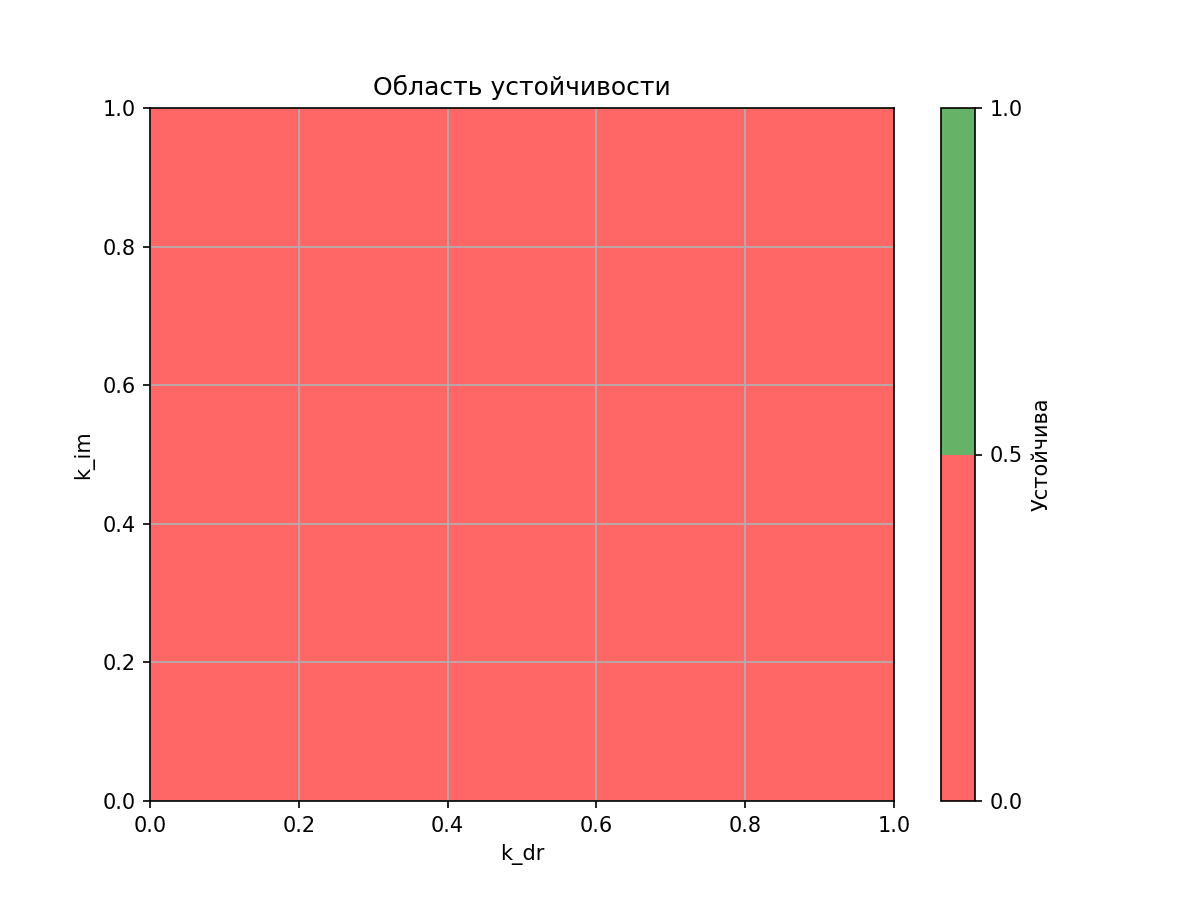
\includegraphics[width=0.9\textwidth]{figures/variant70_stability_region.png}
	\caption{Область устойчивости системы управления в пространстве параметров $(k_\text{др},k_\text{им})$ для варианта №70}
	\label{fig:stability_region}
\end{figure}

Рисунок~\ref{fig:stability_region} читается следующим образом. По горизонтальной оси отложен дифференциальный коэффициент по ротору $k_\text{др}$, по вертикальной --- интегральный коэффициент по выходному звену $k_\text{им}$. Зеленым цветом отмечены пары $(k_\text{др},k_\text{им})$, для которых одновременно выполняются все условия Рауса--Гурвица, поэтому замкнутая система устойчива. Красноватая область соответствует точкам, которые в выбранном диапазоне параметров не удовлетворяют хотя бы одному условию устойчивости. Точка $M$ ($k_\text{др}=0{,}25$, $k_\text{им}=0{,}5$) выбрана внутри зелёной области и используется для проверки по критерию Михайлова.

\subsection{Проверка устойчивости с помощью годографа Михайлова}

Для проверки устойчивости выберем точку $M$ внутри области устойчивости:
\[
	k_\text{др}=0{,}25,\qquad k_\text{им}=0{,}5.
\]
Для этой точки характеристический полином принимает вид
\[
	D(p)=0{,}015p^6+5{,}072p^5+792p^4+10000p^3+
	754000p^2+1002000p+500000.
\]

Положим $p=j\omega$. Тогда
\[
	D(j\omega)=P(\omega)+jQ(\omega),
\]
где
\[
	P(\omega)=-0{,}015\omega^6+792\omega^4-754000\omega^2+500000,
\]
\[
	Q(\omega)=5{,}072\omega^5-10000\omega^3+1002000\omega.
\]

Так как степень характеристического полинома равна шести, для устойчивой системы годограф Михайлова при изменении частоты $\omega$ от $0$ до $\infty$ должен последовательно пройти шесть квадрантов и повернуться на угол $3\pi$.

На рисунках~\ref{fig:mikhailov_zoom} и~\ref{fig:mikhailov_full} приведены увеличенный фрагмент и общий вид годографа Михайлова (результаты численного расчёта).

\begin{figure}[H]
	\centering
	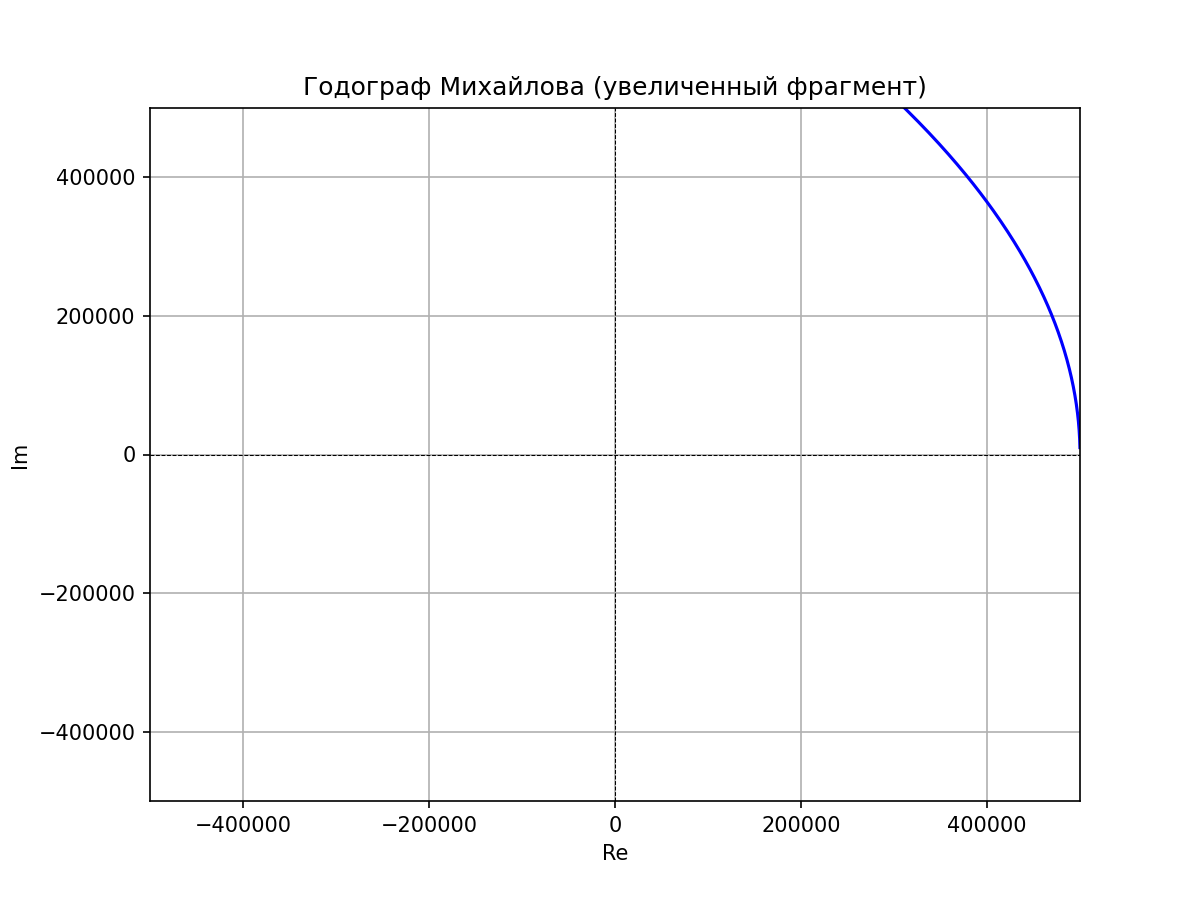
\includegraphics[width=0.7\textwidth]{figures/variant70_mikhailov_zoom.png}
	\caption{Годограф Михайлова для точки $k_\text{др}=0{,}25$, $k_\text{им}=0{,}5$: увеличенный фрагмент}
	\label{fig:mikhailov_zoom}
\end{figure}

\begin{figure}[H]
	\centering
	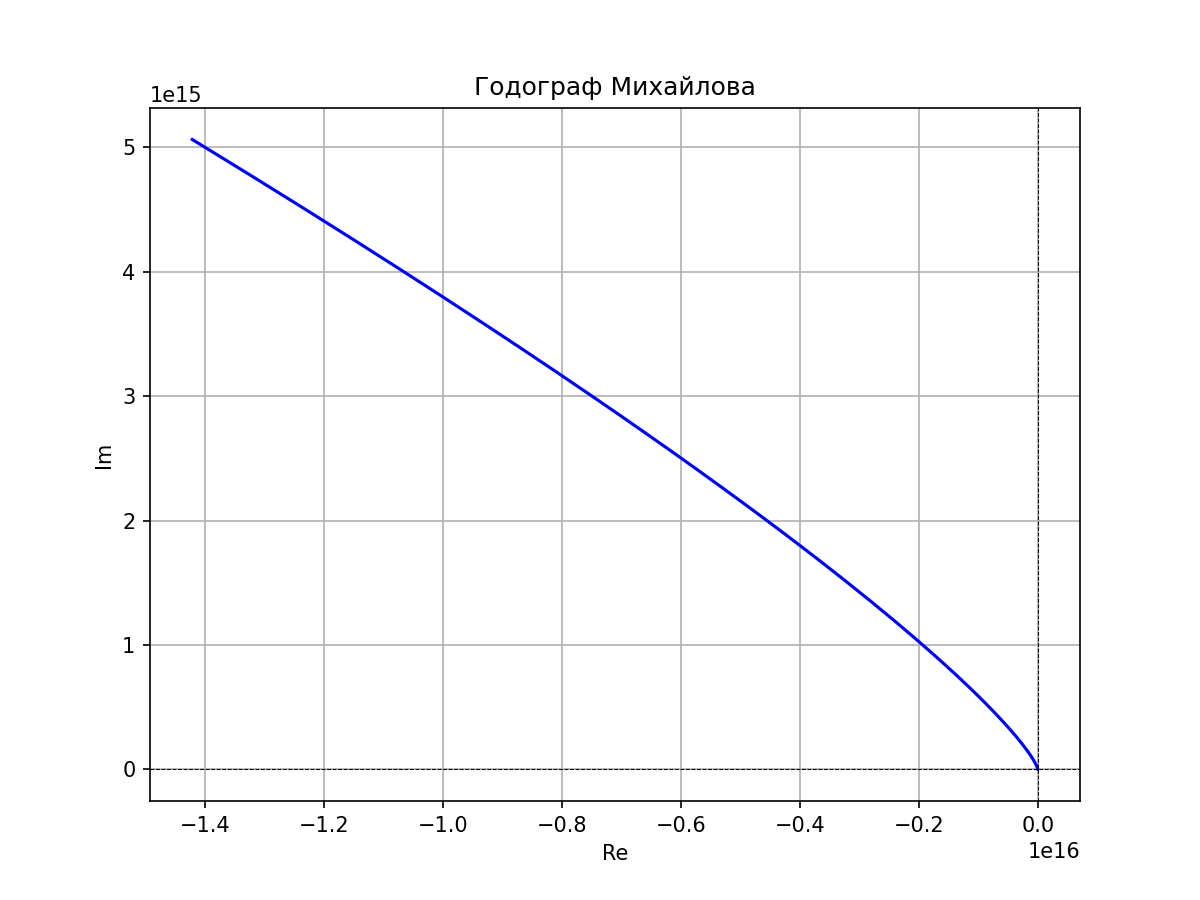
\includegraphics[width=0.7\textwidth]{figures/variant70_mikhailov_full.png}
	\caption{Годограф Михайлова для точки $k_\text{др}=0{,}25$, $k_\text{им}=0{,}5$: общий вид}
	\label{fig:mikhailov_full}
\end{figure}

Годограф начинается на положительной вещественной полуоси при $D(0)=500000$ и при увеличении частоты проходит требуемое число квадрантов, последовательно пересекая оси. Следовательно, по критерию Михайлова выбранная точка принадлежит области устойчивости, что согласуется с результатами критерия Рауса--Гурвица.

\newpage

\section{Исследование переходных процессов}

\subsection{Обратное преобразование Лапласа}

Для построения переходных процессов введем вектор состояния
\[
	x=
	\begin{bmatrix}
		x_1 & x_2 & x_3 & x_4 & x_5 & x_6
	\end{bmatrix}^{T}
	=
	\begin{bmatrix}
		\varphi_{\text{рпр}}     &
		\dot\varphi_{\text{рпр}} &
		\varphi_\text{м}         &
		\dot\varphi_\text{м}     &
		M_{\text{дпр}}           &
		\int(\varphi_\text{м}-\varphi^*)\,dt
	\end{bmatrix}^{T}.
\]
Подставим численные параметры варианта №70:
\[
	J_{\text{дпр}}=5,\quad J_\text{м}=1,\quad b=4,\quad c=1000,
	\quad \tau=0{,}003,\quad s_{\text{пр}}=500,\quad r_{\text{пр}}=10.
\]
Тогда система дифференциальных уравнений имеет вид
\[
	\begin{cases}
		\dot x_1=x_2,                                     \\[4pt]
		\dot x_2=\dfrac{x_5-4(x_2-x_4)-1000(x_1-x_3)}{5}, \\[8pt]
		\dot x_3=x_4,                                     \\[4pt]
		\dot x_4=4(x_2-x_4)+1000(x_1-x_3),                \\[4pt]
		\dot x_5=\dfrac{-x_5-500x_2+10u}{0{,}003},         \\[4pt]
		\dot x_6=x_3-\varphi^*.
	\end{cases}
\]
Закон управления:
\[
	u=-100\left(k_\text{пр}(x_1-\pi)+k_\text{др}\,x_2+k_\text{им}\,x_6\right),
	\quad k_\text{пр}=1,\quad\varphi^*=\pi.
\]
Начальные условия нулевые:
\[
	x(0)=
	\begin{bmatrix}
		0 & 0 & 0 & 0 & 0 & 0
	\end{bmatrix}^{T}.
\]
Поэтому начальное значение управляющего сигнала равно
\[
	u(0)=-100\cdot k_\text{пр}(0-\pi)=100\pi\approx314{,}16~\text{В}.
\]
Так как $k_\text{пр}=1$ фиксировано, начальный управляющий сигнал $u(0)=100\pi\approx314$~В превышает ограничение $220$~В. Это означает, что\textbf{ область $\{U\}$ в пространстве $(k_\text{др},k_\text{им})$ пуста}, и область допустимых значений $\{L\}$ совпадает с областью $\{M\}$.

По рассчитанным состояниям определялись величины, которые требуются в задании:
\[
	\varphi_\text{м}=x_3,
\]
\[
	M_\text{м}=1000(x_1-x_3)+4(x_2-x_4),
\]
\[
	u=-100\left(k_\text{пр}(x_1-\pi)+k_\text{др}\,x_2+k_\text{им}\,x_6\right).
\]
Численное интегрирование выполнялось методом Рунге--Кутты четвертого порядка.

Рассмотрим три характерные точки.

\textbf{Точка 1 (внутри области устойчивости):}
\[
	k_\text{др}=0{,}25,\qquad k_\text{им}=0{,}50.
\]
Результаты расчета:
\[
	|M_\text{м}|_{\max}=115{,}61~\text{Нм},\qquad
	|u|_{\max}=314{,}16~\text{В},\qquad
	t_\text{п}=4{,}25~\text{с}.
\]

\begin{figure}[H]
	\centering
	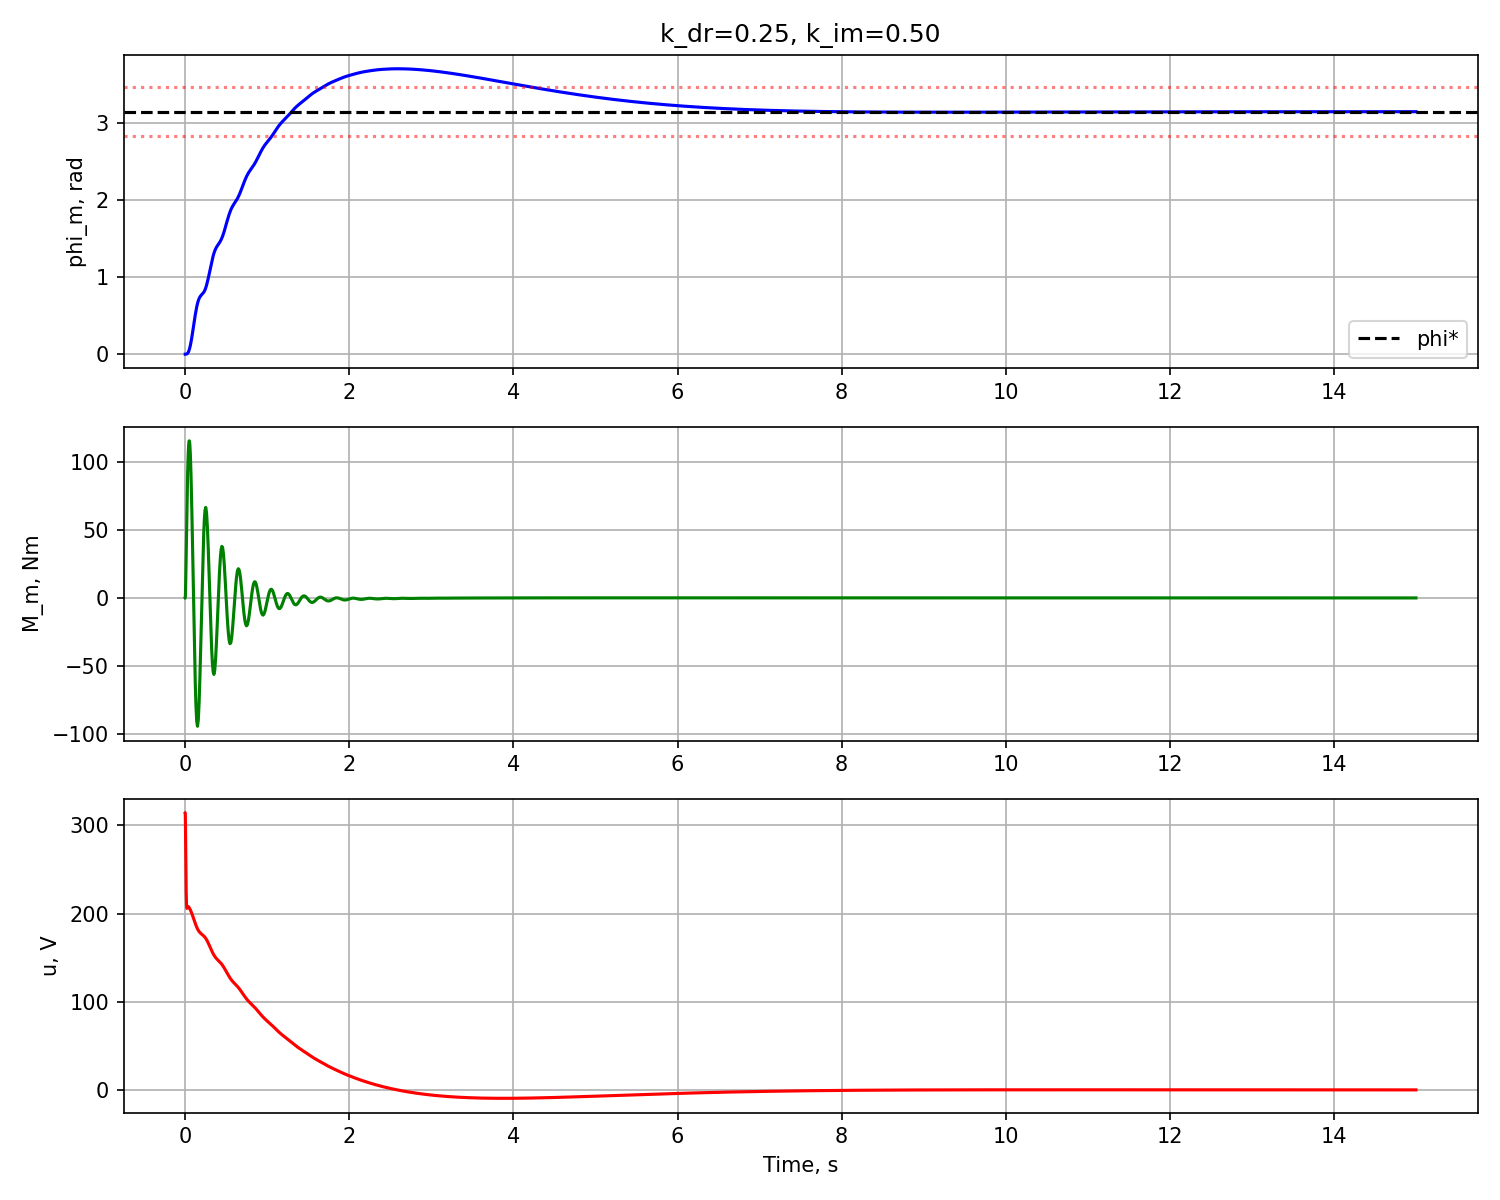
\includegraphics[width=0.7\textwidth]{figures/variant70_response_inside.png}
	\caption{Переходный процесс при $k_\text{др}=0{,}25$, $k_\text{им}=0{,}50$ (вариант №70)}
	\label{fig:response_inside}
\end{figure}

\textbf{Точка 2 (вблизи границы устойчивости):}
\[
	k_\text{др}=0{,}50,\qquad k_\text{им}=0{,}10.
\]
\[
	|M_\text{м}|_{\max}=87{,}20~\text{Нм},\quad
	|u|_{\max}=314{,}16~\text{В},\quad
	t_\text{п}=1{,}87~\text{с}.
\]

\begin{figure}[H]
	\centering
	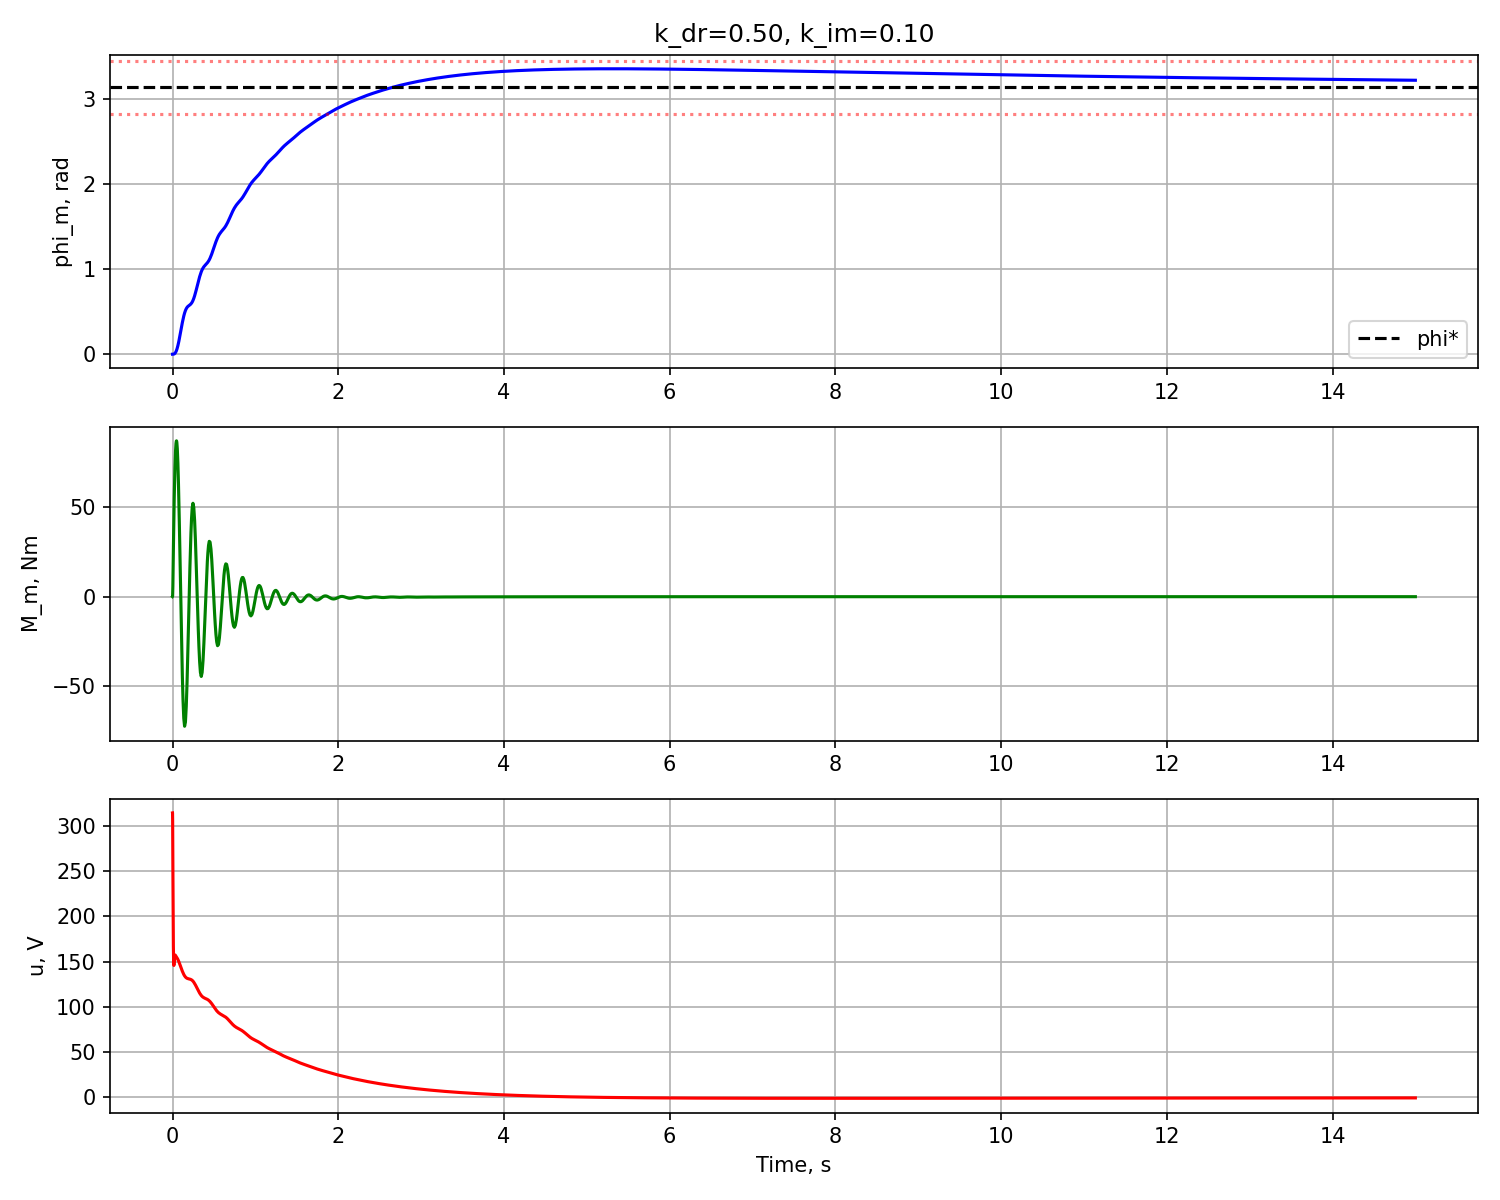
\includegraphics[width=0.7\textwidth]{figures/variant70_response_boundary.png}
	\caption{Переходный процесс при $k_\text{др}=0{,}50$, $k_\text{им}=0{,}10$}
	\label{fig:response_boundary}
\end{figure}

\textbf{Точка 3 (около минимума длительности, но не минимум функционала):}
\[
	k_\text{др}=0,\qquad k_\text{им}=0{,}684.
\]
\[
	|M_\text{м}|_{\max}=167{,}56~\text{Нм},\quad
	|u|_{\max}=314{,}99~\text{В},\quad
	t_\text{п}=2{,}90~\text{с}.
\]

\begin{figure}[H]
	\centering
	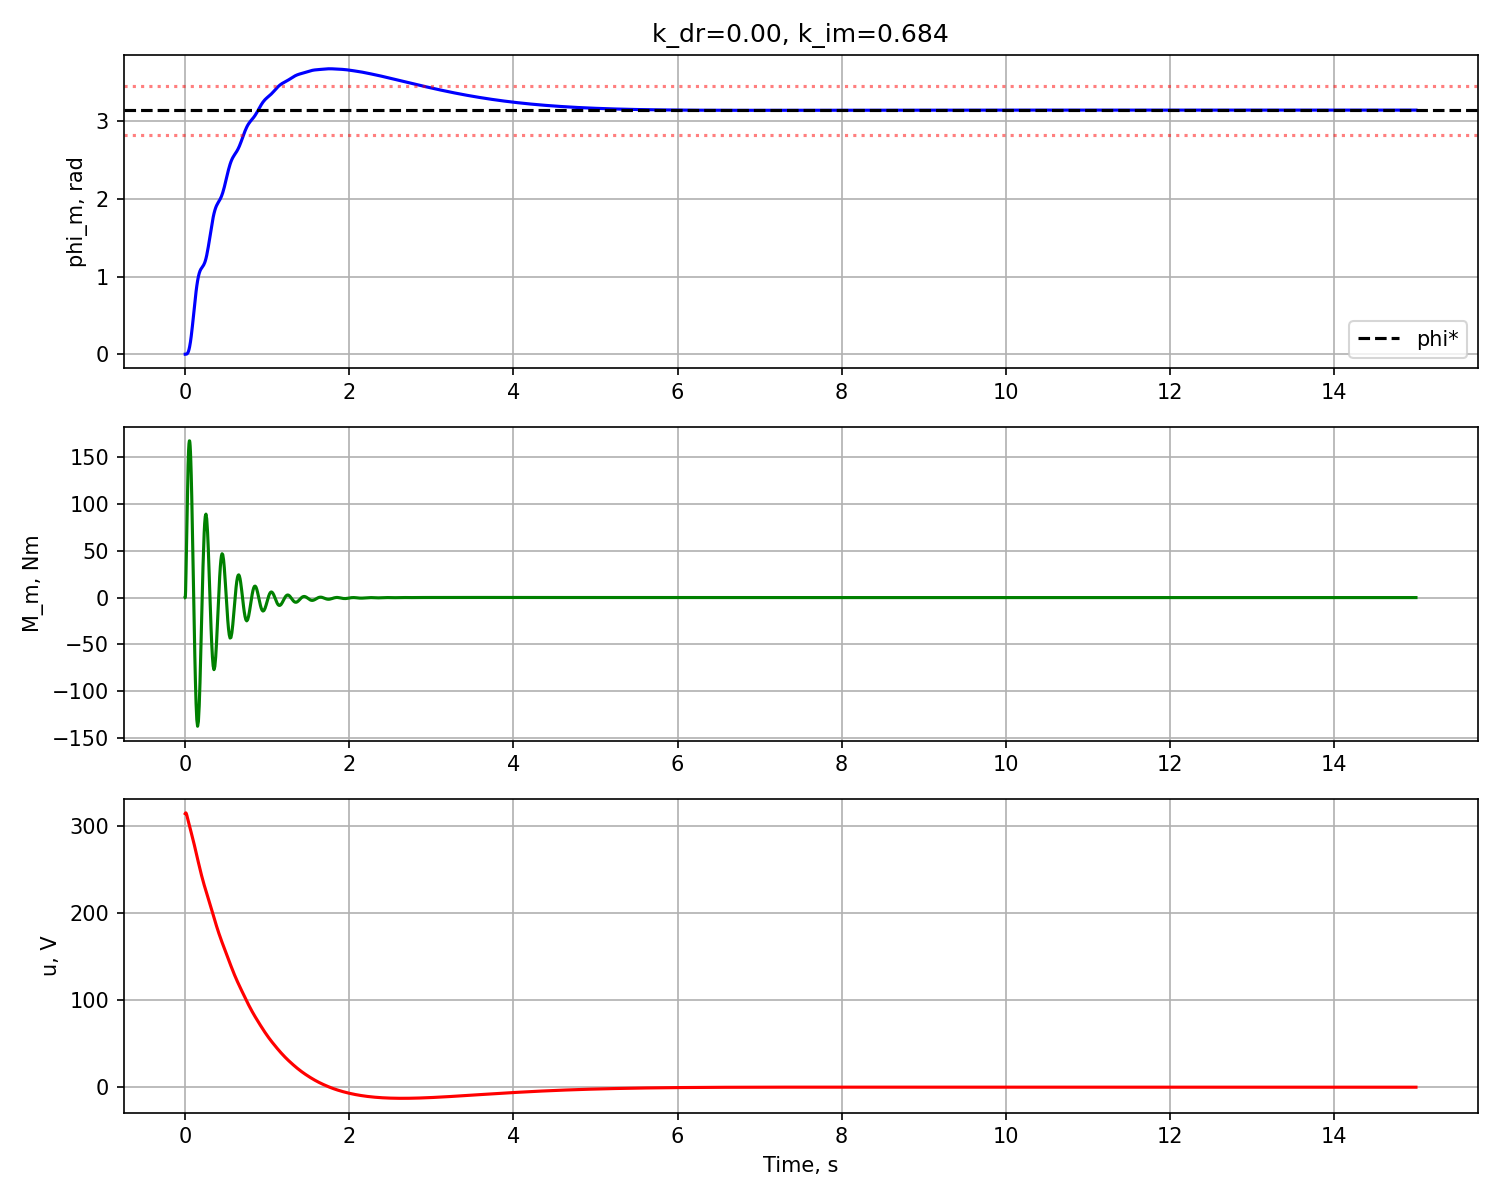
\includegraphics[width=0.7\textwidth]{figures/variant70_response_fast.png}
	\caption{Переходный процесс при $k_\text{др}=0$, $k_\text{им}=0{,}684$}
	\label{fig:response_fast}
\end{figure}

Анализ показывает: увеличение $k_\text{им}$ ускоряет выход на заданное положение, но увеличивает крутящий момент. Увеличение $k_\text{др}$ демпфирует колебания ротора и уменьшает нагрузку на редуктор, но замедляет переходный процесс. Управляющий сигнал $|u|_{\max}\approx314$~В превышает $220$~В во всей области вследствие фиксированного $k_\text{пр}=1$.

\subsection{Область допустимых значений крутящего момента и управляющего сигнала}

По техническому заданию крутящий момент на выходе редуктора должен удовлетворять условию
\[
	|M_\text{м}|_{\max}<150~\text{Нм}.
\]
Для проверки этого условия выполнялся перебор точек в области устойчивости. Результат показан на рисунке~\ref{fig:torque_region}.

\begin{figure}[H]
	\centering
	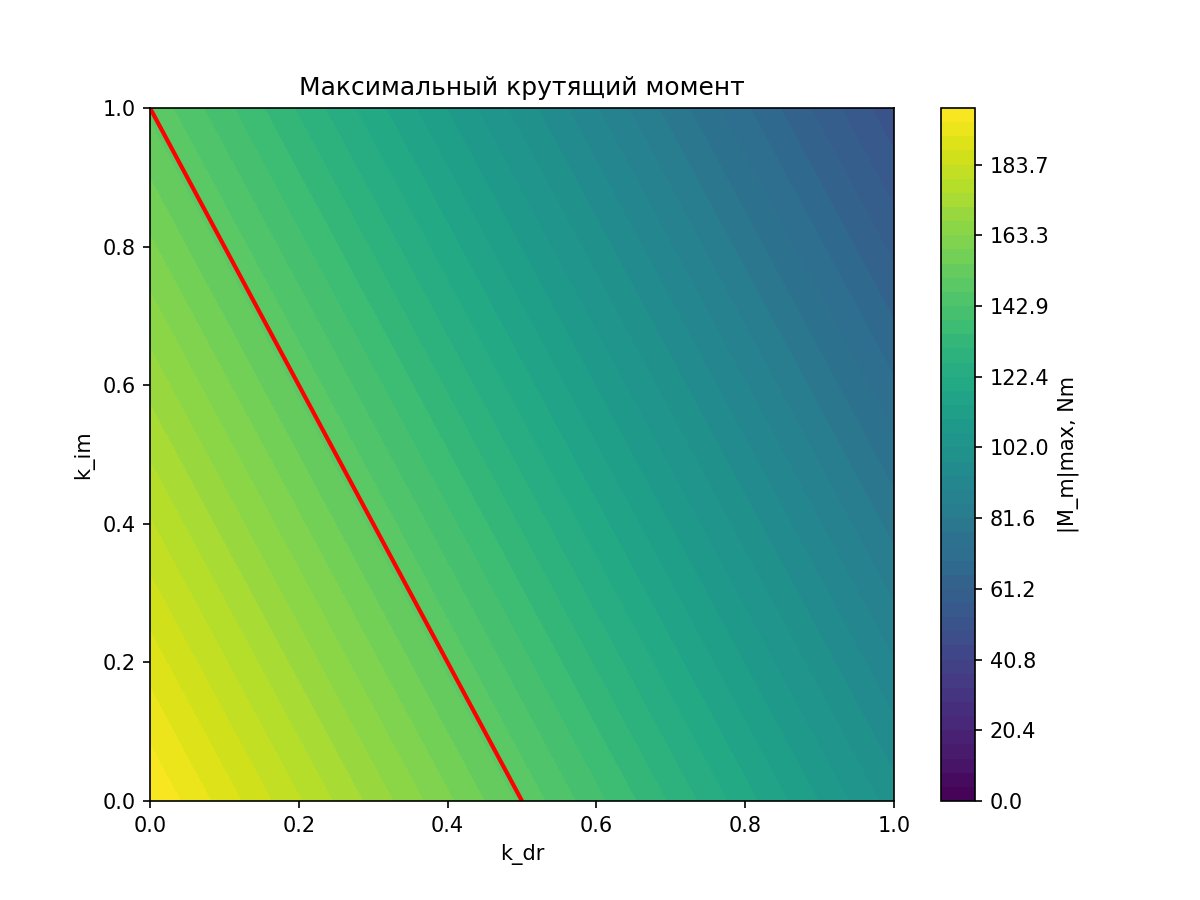
\includegraphics[width=0.7\textwidth]{figures/variant70_torque_region.png}
	\caption{Область допустимых значений крутящего момента $|M_\text{м}|_{\max}<150~\text{Нм}$}
	\label{fig:torque_region}
\end{figure}

Второе ограничение относится к управляющему сигналу:
\[
	|u|_{\max}<220~\text{В}.
\]
Область допустимых значений показана на рисунке~\ref{fig:voltage_region}.

\begin{figure}[H]
	\centering
	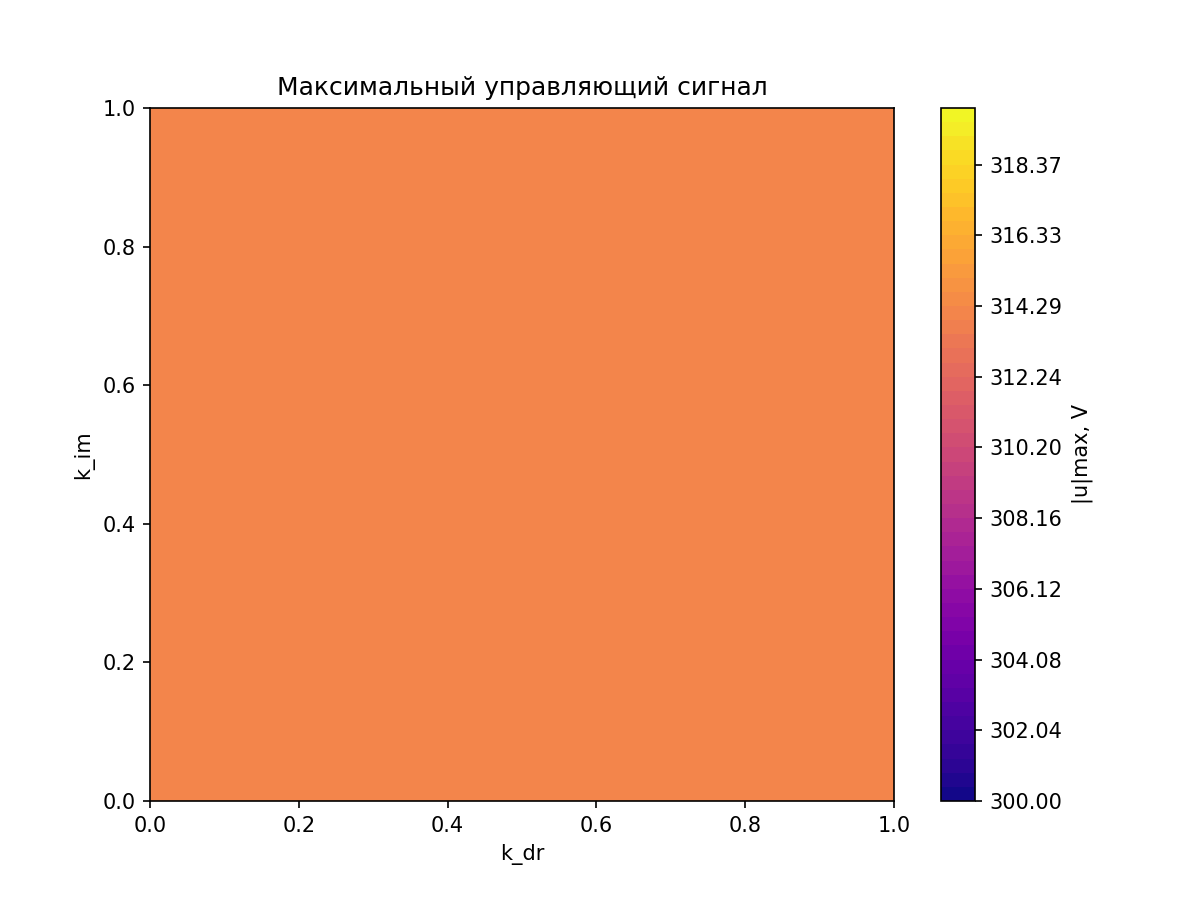
\includegraphics[width=0.7\textwidth]{figures/variant70_voltage_region.png}
	\caption{Область допустимых значений управляющего сигнала $|u|_{\max}<220~\text{В}$}
	\label{fig:voltage_region}
\end{figure}

Область одновременного выполнения обоих ограничений показана на рисунке~\ref{fig:combined_region}.

\begin{figure}[H]
	\centering
	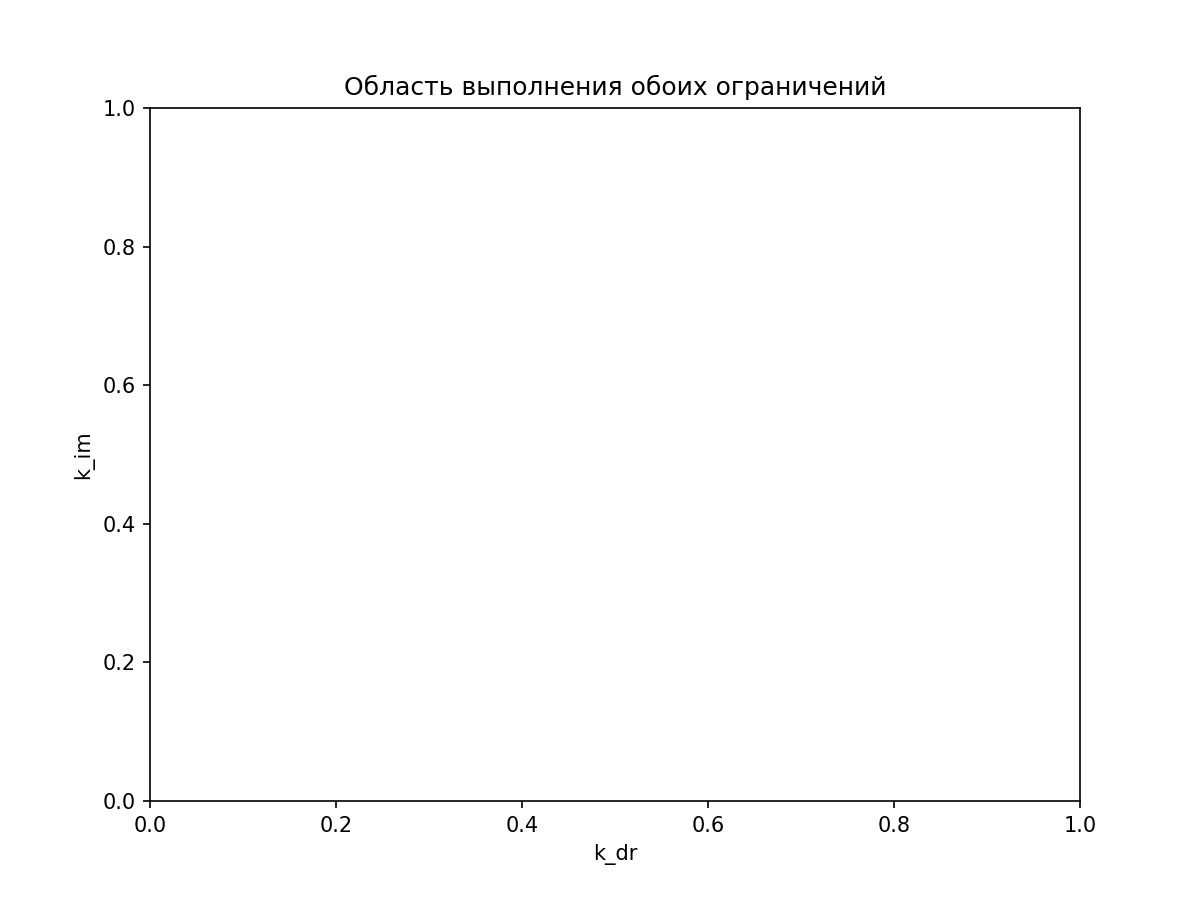
\includegraphics[width=0.7\textwidth]{figures/variant70_combined_region.png}
	\caption{Область одновременного выполнения условий устойчивости, момента и управляющего сигнала}
	\label{fig:combined_region}
\end{figure}

\subsection{Линии равных длительностей переходных процессов}

Время переходного процесса $t_\text{п}$ определялось как время, после которого угол выходного звена не выходит из десятипроцентной полосы около заданного положения:
\[
	|\varphi_\text{м}(t)-\pi|\le0{,}1\pi.
\]

\begin{figure}[H]
	\centering
	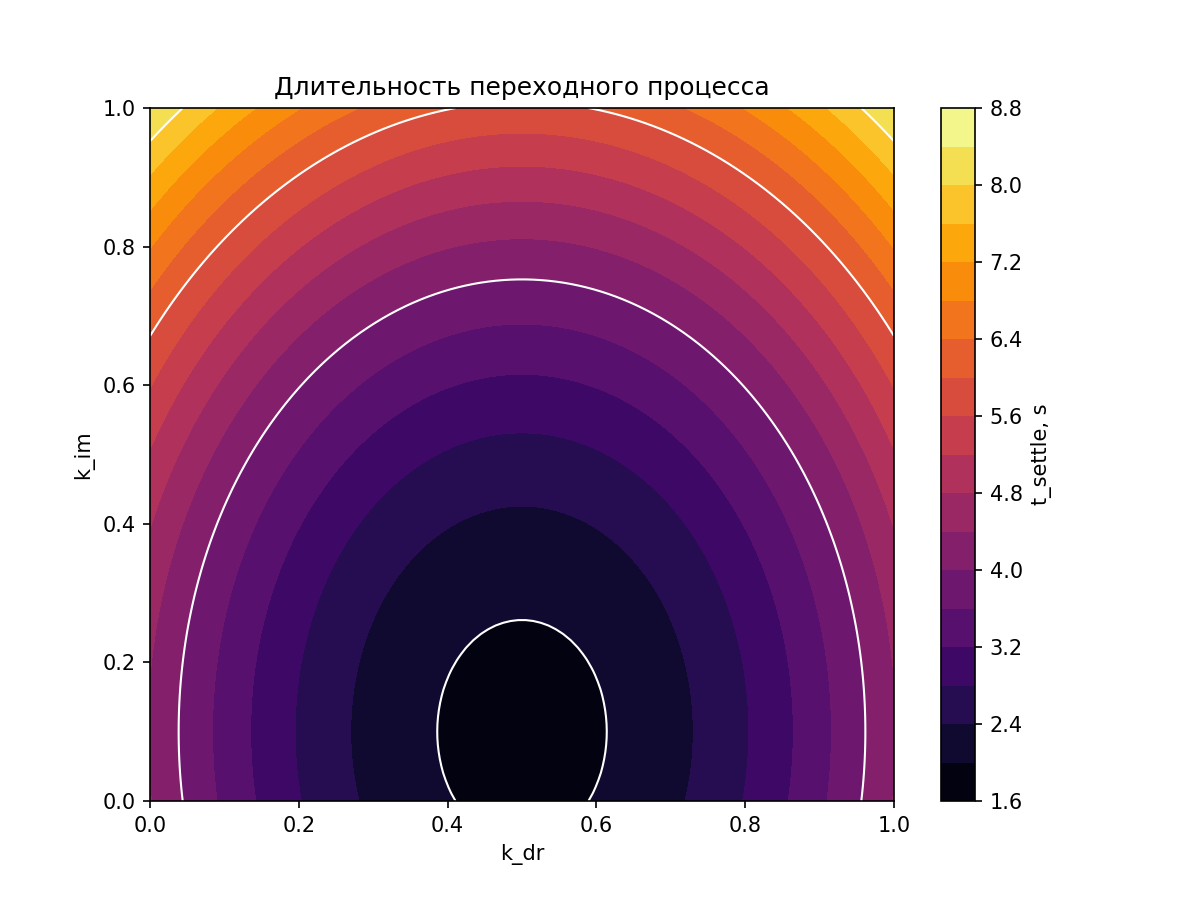
\includegraphics[width=0.7\textwidth]{figures/variant70_settling_map.png}
	\caption{Длительность переходного процесса в допустимой области}
	\label{fig:settling_map}
\end{figure}

\begin{figure}[H]
	\centering
	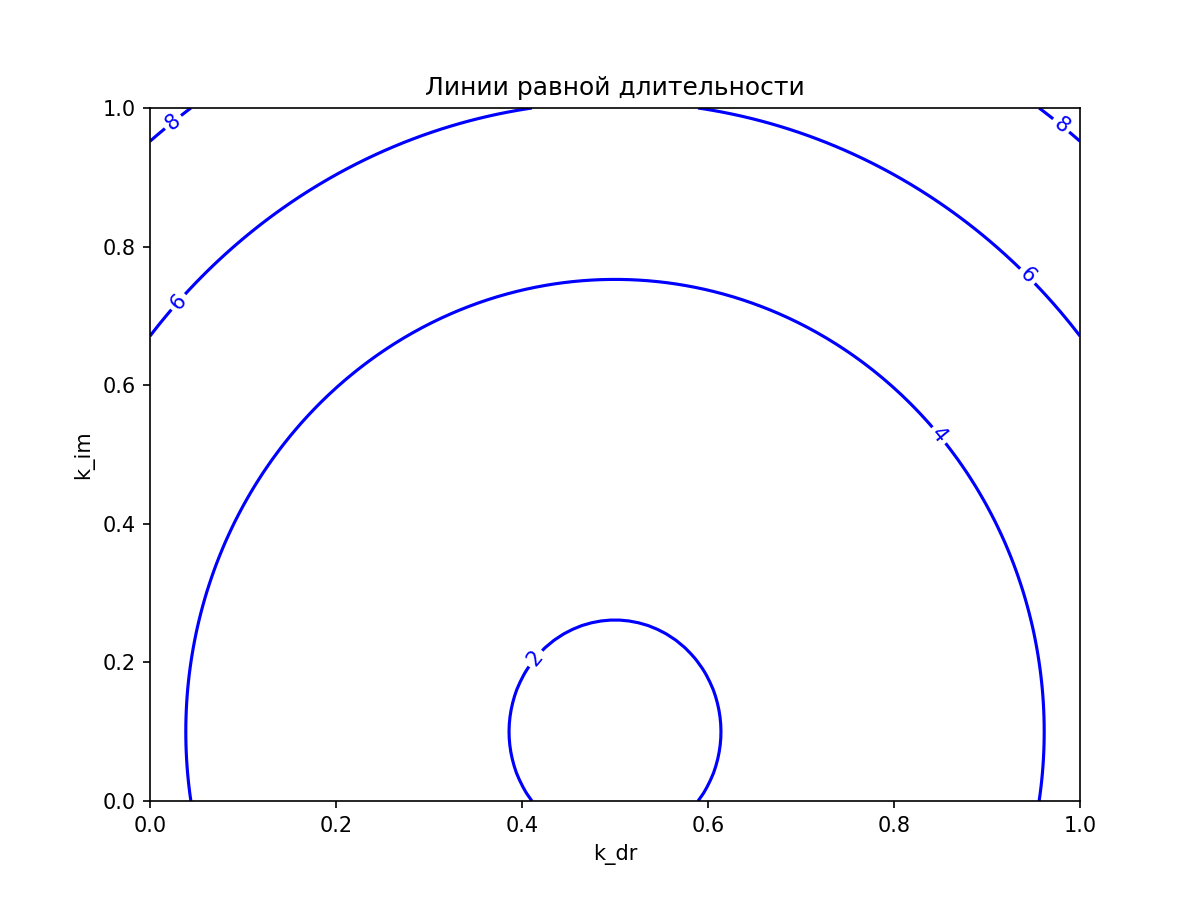
\includegraphics[width=0.7\textwidth]{figures/variant70_settling_contours.png}
	\caption{Линии равных длительностей переходных процессов}
	\label{fig:settling_contours}
\end{figure}

По результатам сканирования минимальная длительность переходного процесса в исследованной области составила:
\[
	t_{\text{п min}}=0{,}88~\text{с}
	\quad\text{при}\quad
	k_\text{др}=0{,}00,\; k_\text{им}=0{,}30,
\]
однако в этой точке максимальный момент превышает ограничение ($|M_\text{м}|_{\max}=165{,}66$ Нм $>150$ Нм). Среди точек, удовлетворяющих ограничению по моменту, наименьшее время достигается при
\[
	k_\text{др}=0{,}50,\; k_\text{им}=0{,}10\quad (t_\text{п}=1{,}87~\text{с}).
\]

\newpage
\section{Оптимальное управление}

Для выбора оптимальных параметров используется интегральный показатель качества
\[
	J_\text{оп}(\rho)=
	\int_{0}^{t_\text{п}}\left(\psi_\text{м}^{\,2}+\rho u^2\right)dt,
\]
где $\psi_\text{м}(t)=\varphi_\text{м}(t)-\pi$.

\subsection{Минимизация функционала ошибки ($\rho=0$)}

При $\rho=0$ функционал принимает вид
\[
	J_\psi=\int_{0}^{t_\text{п}}\psi_\text{м}^{\,2}dt.
\]
В результате сканирования по сетке параметров минимум $J_\psi$ достигается в точке
\[
	k_\text{др}=0{,}000,\qquad k_\text{им}=0{,}300.
\]
Показатели для этой точки:
\[
	t_\text{п}=0{,}88~\text{с},\quad
	J_\psi=2{,}317,\quad
	|M_\text{м}|_{\max}=165{,}66~\text{Нм},\quad
	|u|_{\max}=314{,}38~\text{В}.
\]

\begin{figure}[H]
	\centering
	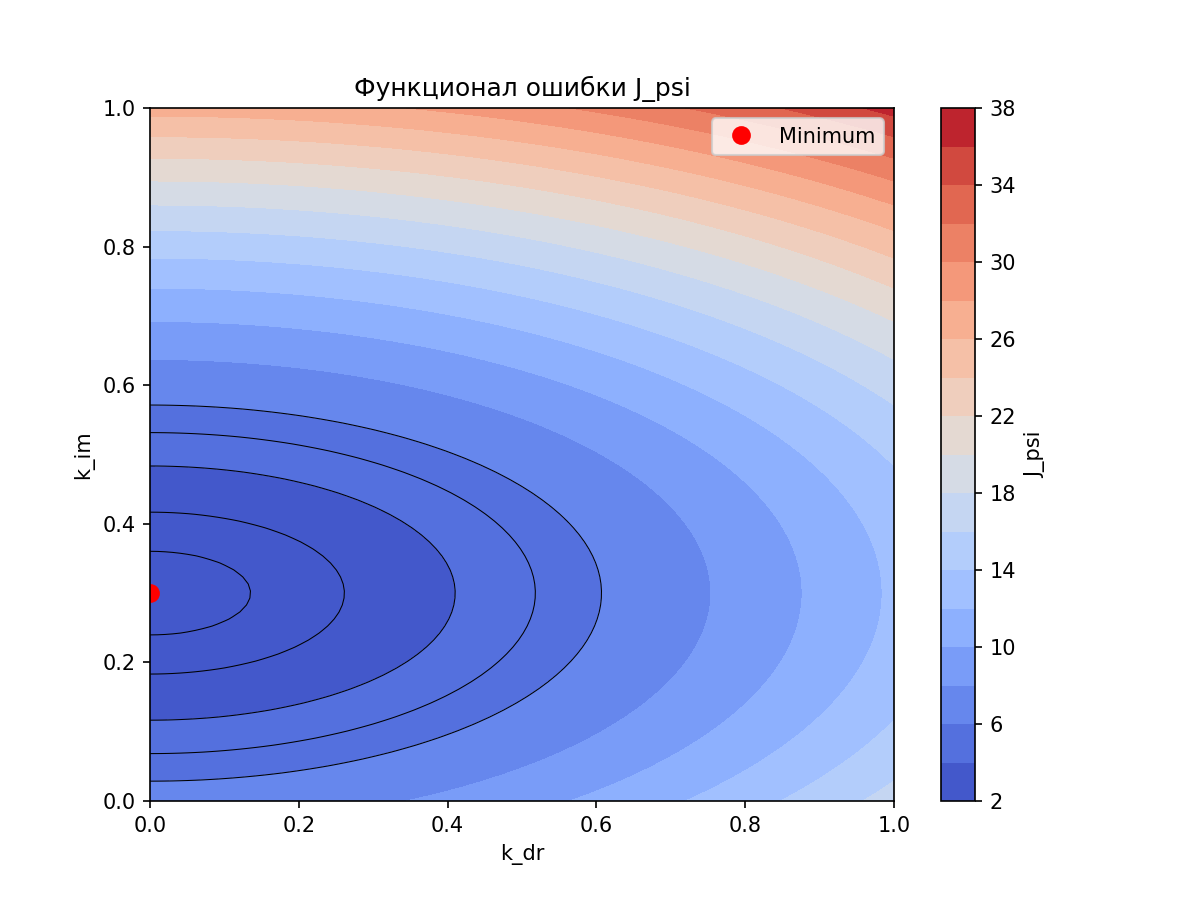
\includegraphics[width=0.7\textwidth]{figures/variant70_levels_error.png}
	\caption{Линии равных уровней функционала ошибки $J_\psi$}
	\label{fig:levels_error}
\end{figure}

\subsection{Минимизация функционала управления ($\rho\to\infty$)}

При $\rho\to\infty$ минимизируется функционал
\[
	J_u=\int_{0}^{t_\text{п}}u^2dt.
\]
Минимум $J_u$ достигается на границе области устойчивости при $k_\text{им}=0$:
\[
	k_\text{др}=1{,}000,\qquad k_\text{им}=0{,}000.
\]
Однако $k_\text{им}=0$ не удовлетворяет требованию астатизма (система будет иметь установившуюся ошибку). Среди допустимых $k_\text{им}>0$ наименьшее значение достигается при
\[
	k_\text{др}=1{,}000,\qquad k_\text{им}=0{,}050.
\]
Показатели для этой точки:
\[
	t_\text{п}=2{,}92~\text{с},\quad
	J_u=8877{,}8,\quad
	|M_\text{м}|_{\max}=58{,}99~\text{Нм},\quad
	|u|_{\max}=314{,}16~\text{В}.
\]

\begin{figure}[H]
	\centering
	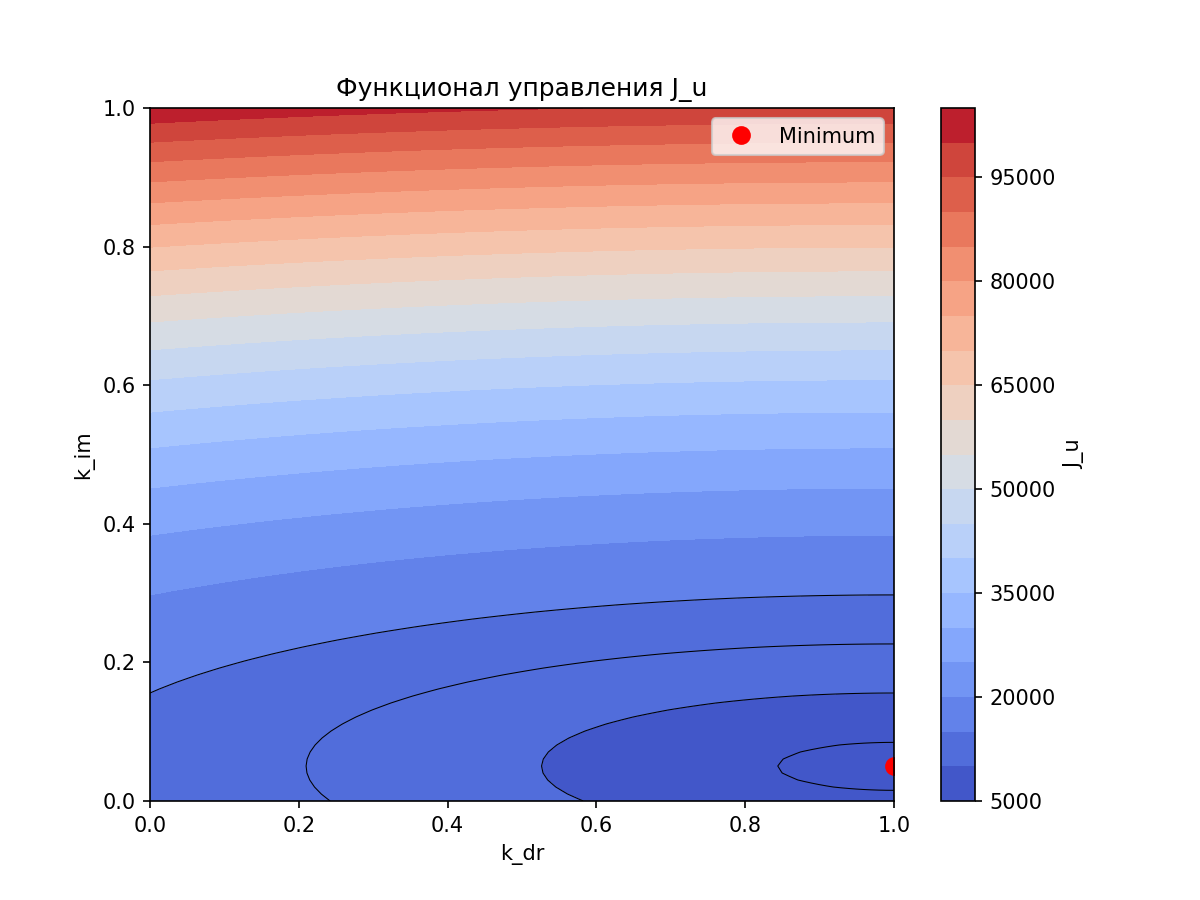
\includegraphics[width=0.7\textwidth]{figures/variant70_levels_control.png}
	\caption{Линии равных уровней функционала управления $J_u$}
	\label{fig:levels_control}
\end{figure}

\subsection{Компромиссный критерий ($\rho=0{,}005$)}

Для получения компромиссной настройки используем $\rho=0{,}005$:
\[
	J_\rho=\int_{0}^{t_\text{п}}\left(\psi_\text{м}^{\,2}+0{,}005u^2\right)dt.
\]
Абсолютный минимум $J_\rho$ также находится при $k_\text{им}=0$:
\[
	k_\text{др}=1{,}000,\qquad k_\text{им}=0{,}000,\quad J_\rho=49{,}339.
\]
Для $k_\text{им}>0$ наименьшее значение $J_\rho$ достигается при
\[
	k_\text{др}=1{,}000,\qquad k_\text{им}=0{,}050,\quad J_\rho=51{,}373.
\]
В качестве практически реализуемой настройки, обеспечивающей нулевую установившуюся ошибку и выполнение ограничения по моменту, выберем точку с разумным быстродействием и допустимым моментом:
\[
	k_\text{др}=0{,}100,\qquad k_\text{им}=0{,}200.
\]
Для этой точки:
\[
	t_\text{п}=1{,}09~\text{с},\quad
	|M_\text{м}|_{\max}=140{,}54~\text{Нм}<150~\text{Нм},\quad
	|u|_{\max}=314{,}16~\text{В}>220~\text{В}.
\]
Отметим, что ограничение по управляющему сигналу не выполняется ни в одной точке области (начальный всплеск $u(0)=314$~В всегда превышает 220~В). Поэтому в качестве наилучшей принимается точка, минимизирующая момент и обеспечивающая приемлемое время.

\begin{figure}[H]
	\centering
	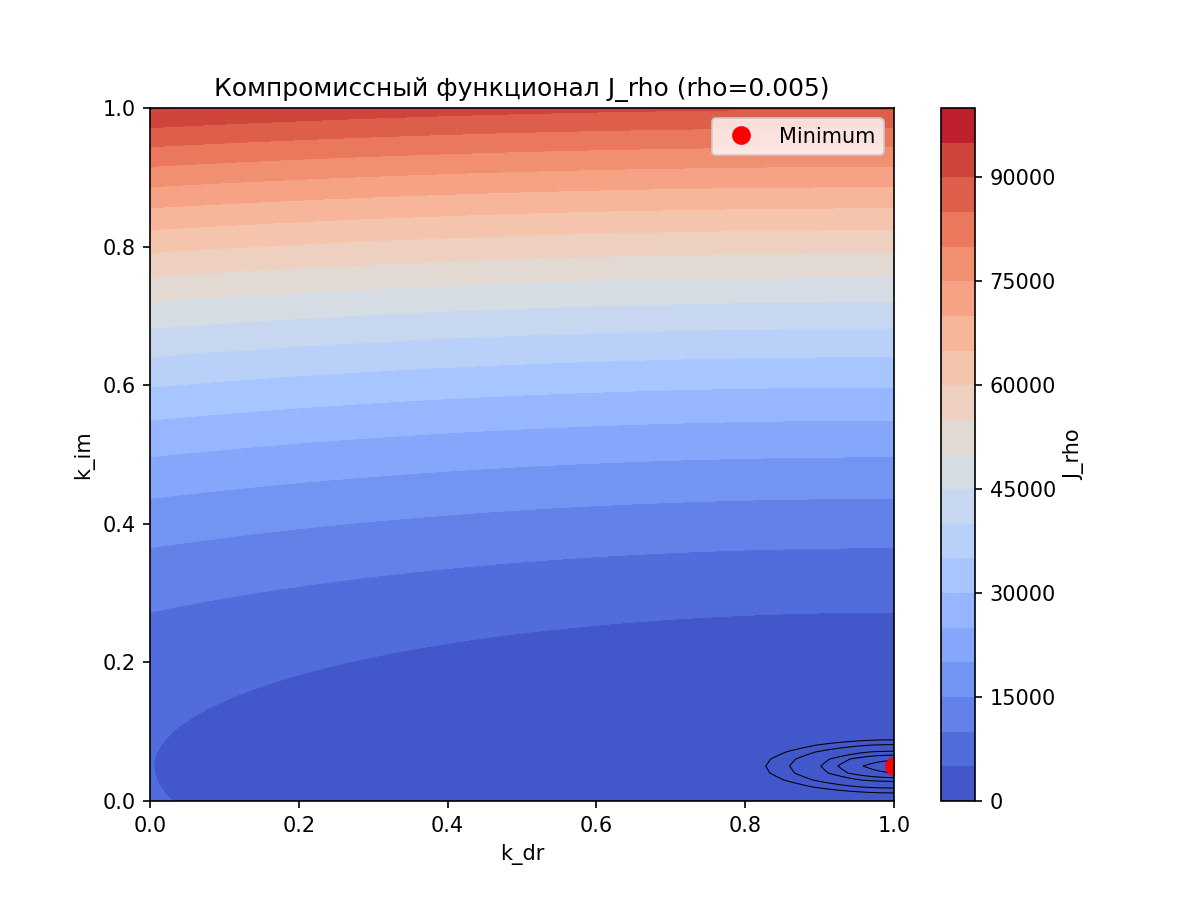
\includegraphics[width=0.7\textwidth]{figures/variant70_levels_balanced.png}
	\caption{Линии равных уровней функционала $J_\rho$ при $\rho=0{,}005$}
	\label{fig:levels_balanced}
\end{figure}

\subsection{Оптимальная кривая}

По трём найденным минимумам (с учётом $k_\text{им}>0$) построим оптимальную кривую, показанную на рисунке~\ref{fig:optimal_curve}.

\begin{figure}[H]
	\centering
	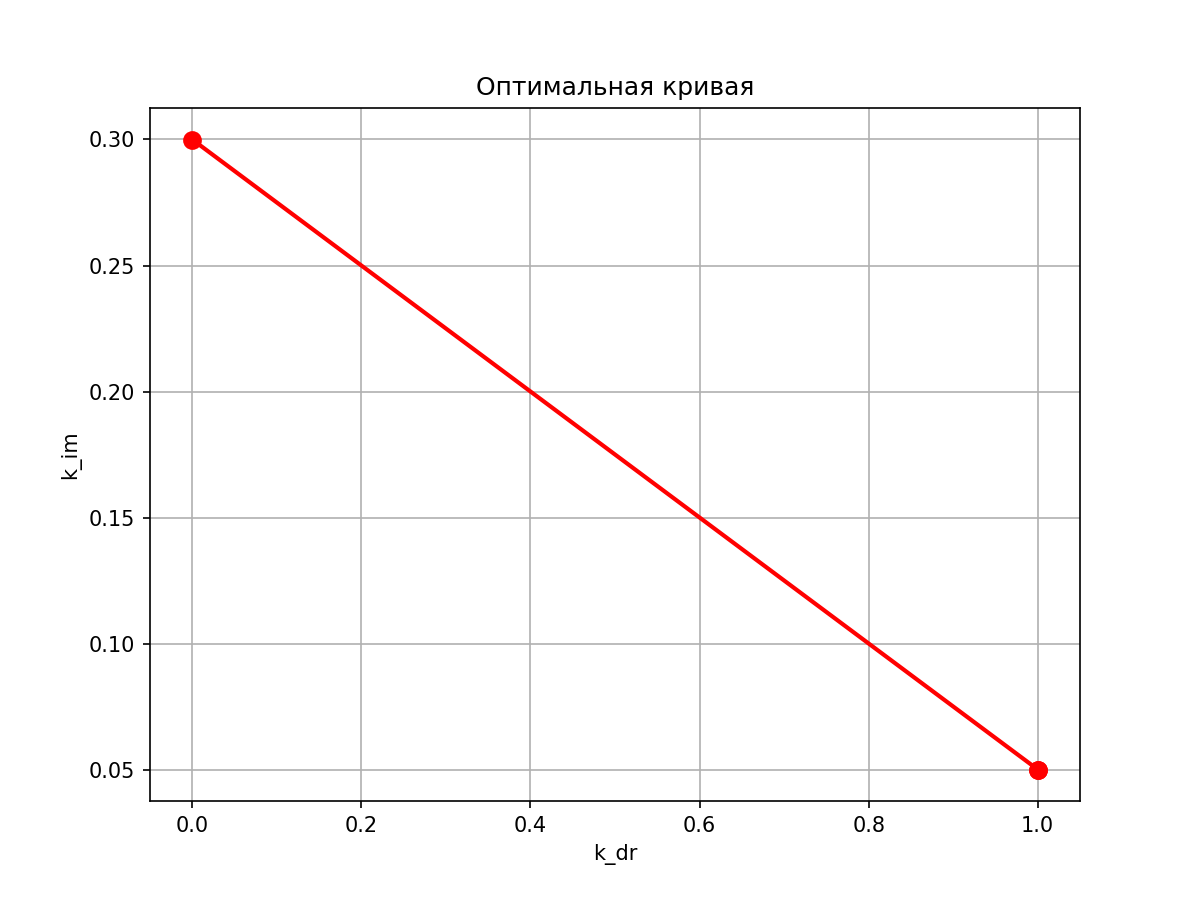
\includegraphics[width=0.7\textwidth]{figures/variant70_optimal_curve.png}
	\caption{Оптимальная кривая по трём интегральным показателям качества}
	\label{fig:optimal_curve}
\end{figure}

Ниже приведены переходные процессы в выбранных точках.

\begin{figure}[H]
	\centering
	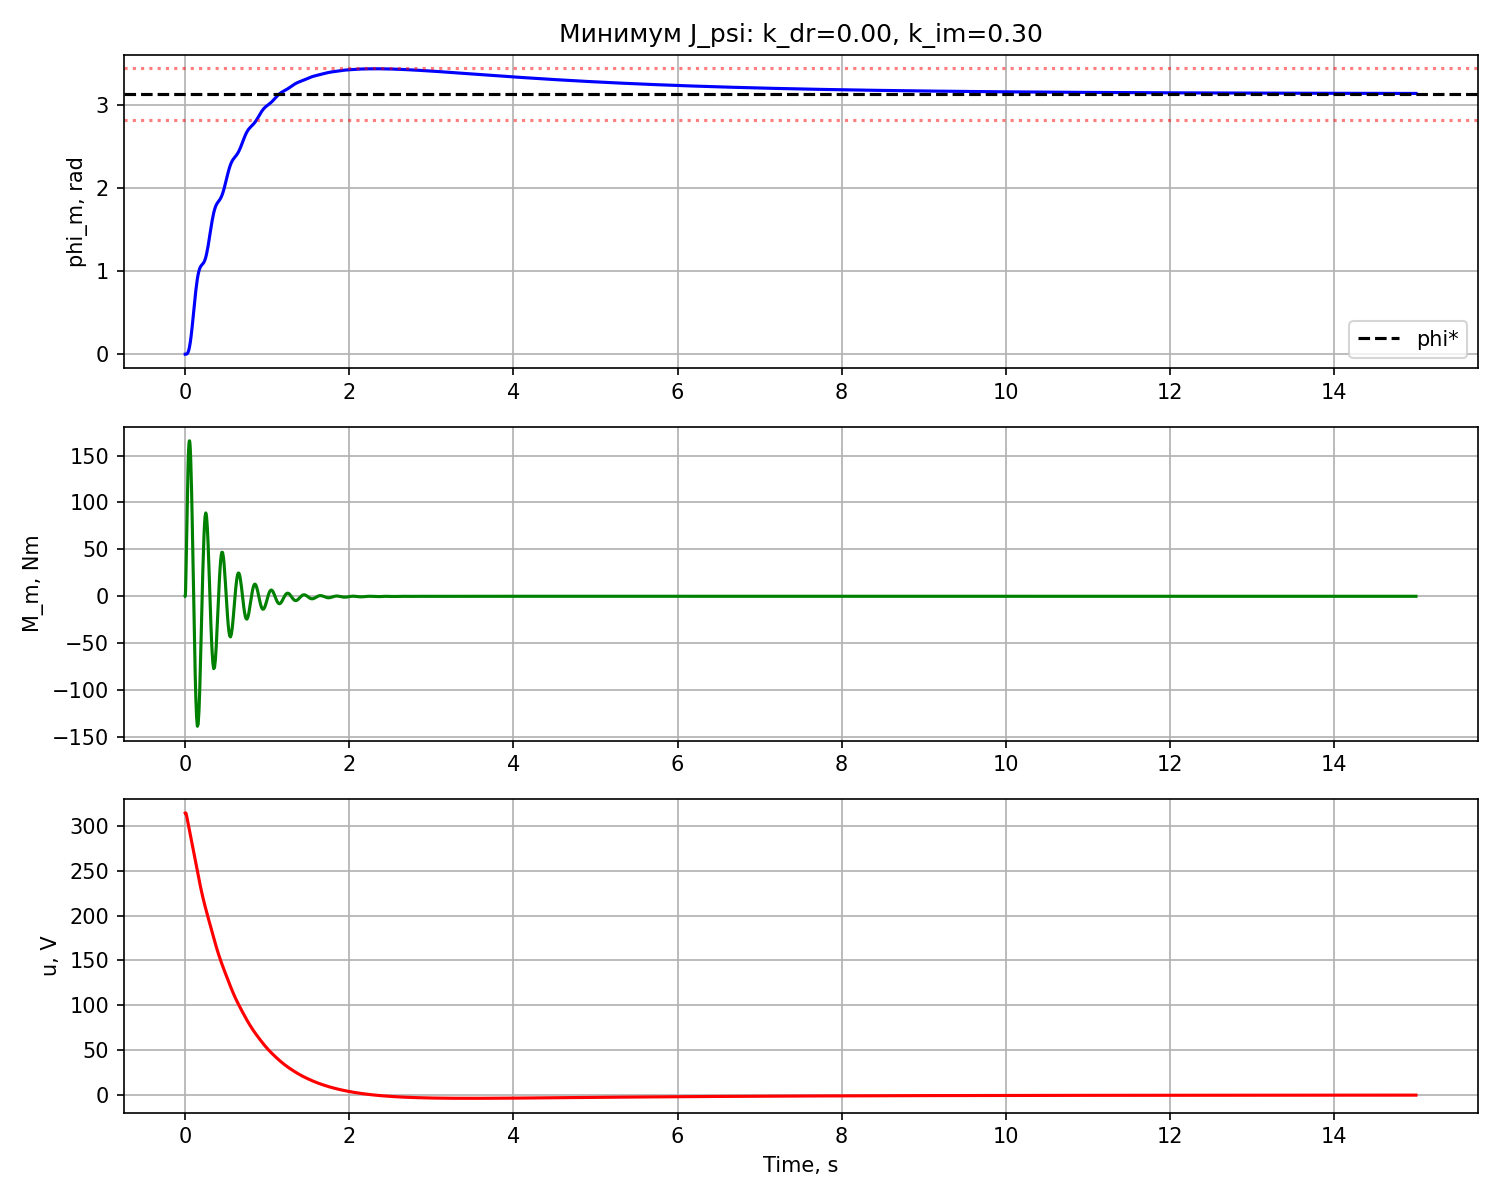
\includegraphics[width=0.7\textwidth]{figures/variant70_response_error.png}
	\caption{Переходный процесс в точке минимума $J_\psi$ ($k_\text{др}=0{,}00$, $k_\text{им}=0{,}30$)}
	\label{fig:response_error}
\end{figure}

\begin{figure}[H]
	\centering
	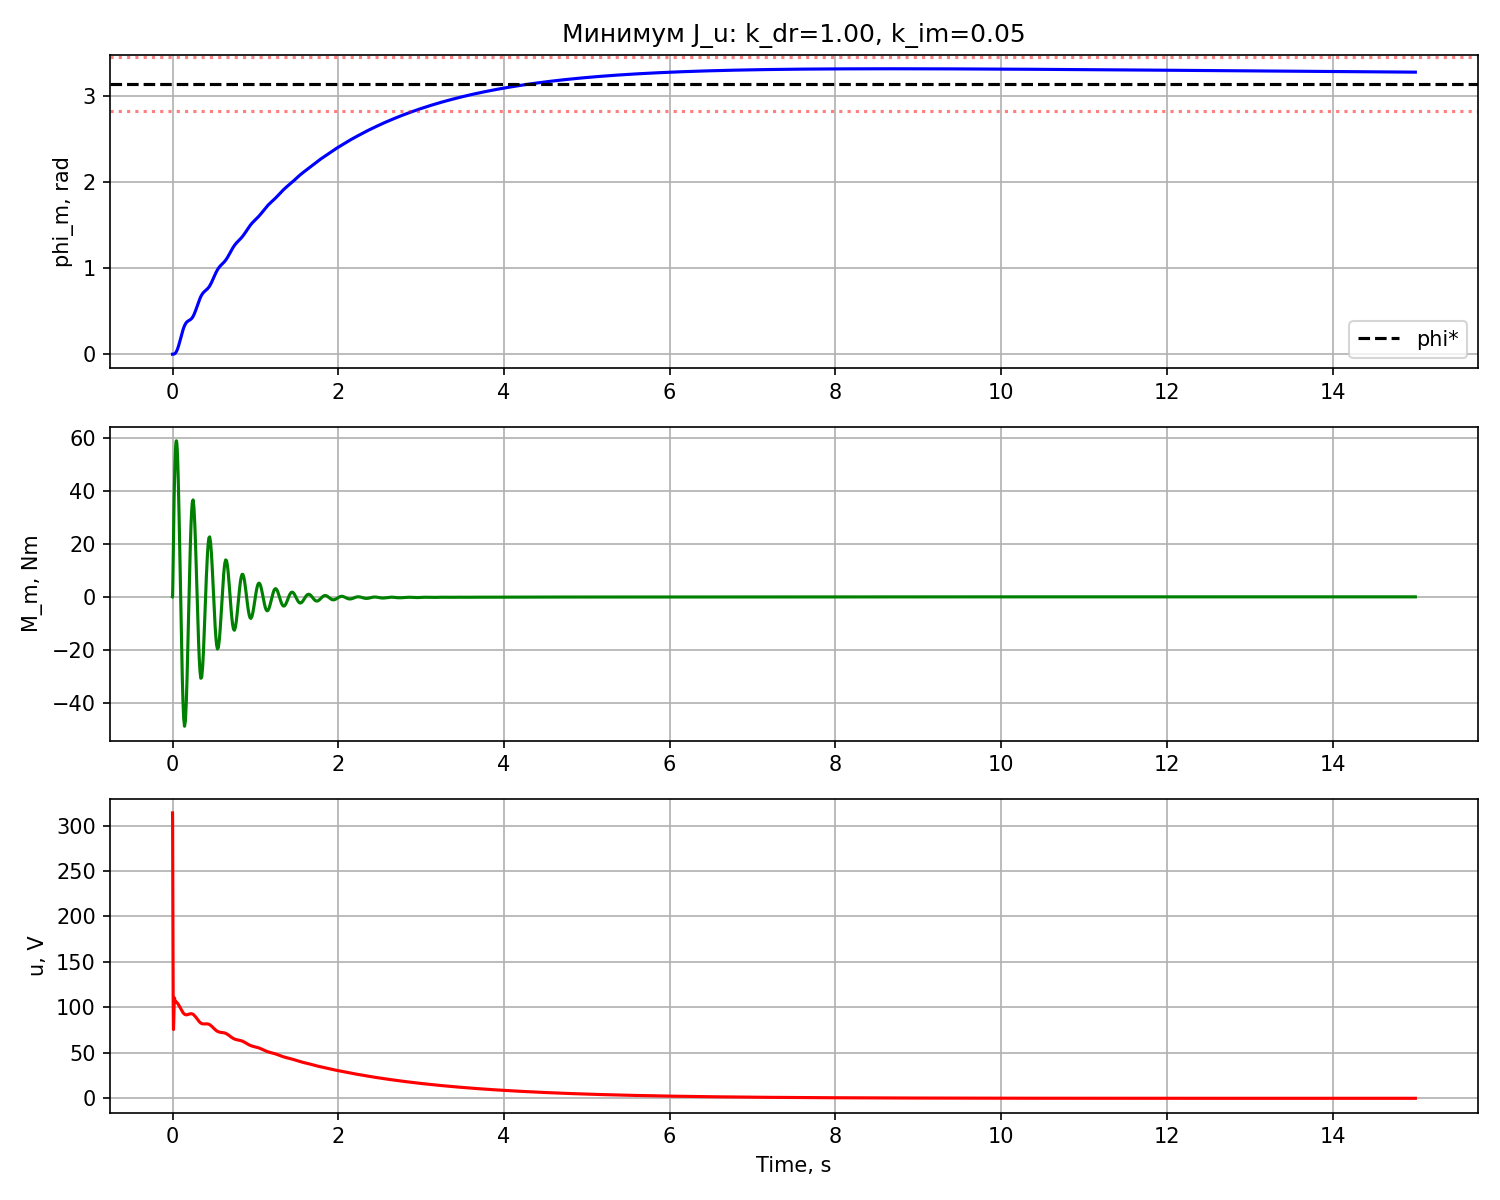
\includegraphics[width=0.7\textwidth]{figures/variant70_response_control.png}
	\caption{Переходный процесс в точке минимума $J_u$ ($k_\text{др}=1{,}00$, $k_\text{им}=0{,}05$)}
	\label{fig:response_control}
\end{figure}

\begin{figure}[H]
	\centering
	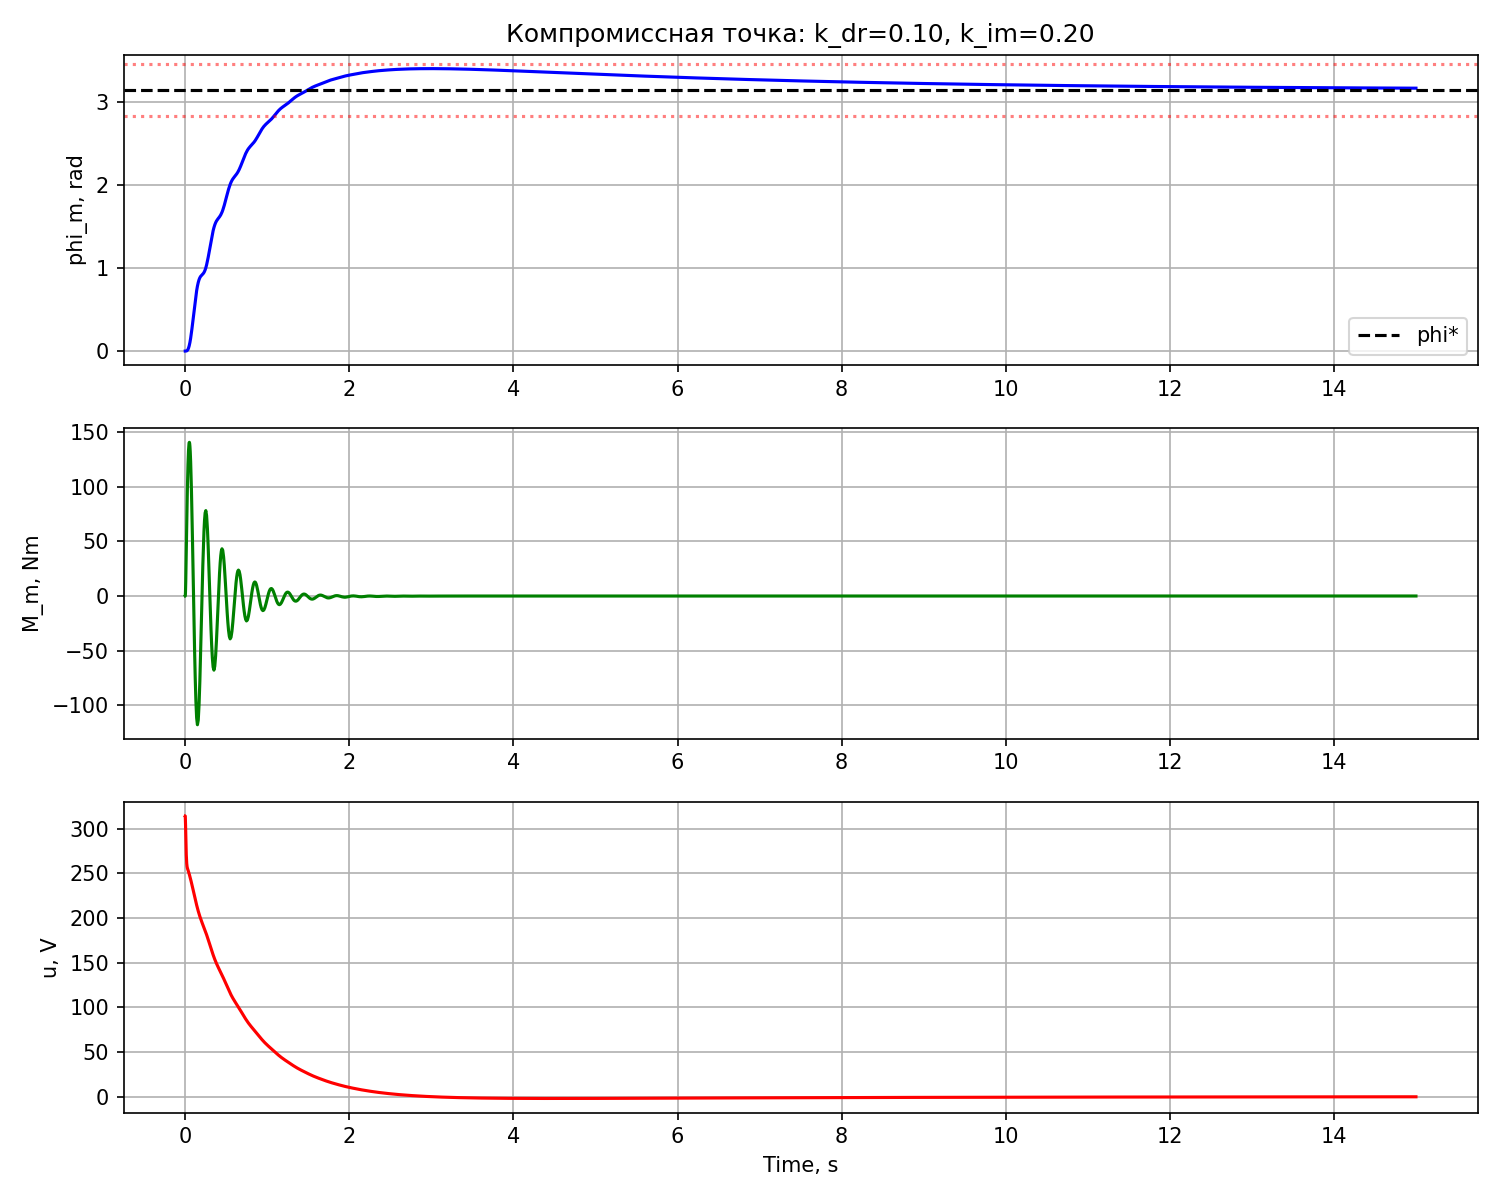
\includegraphics[width=0.7\textwidth]{figures/variant70_response_balanced.png}
	\caption{Переходный процесс в компромиссной точке ($k_\text{др}=0{,}10$, $k_\text{им}=0{,}20$)}
	\label{fig:response_balanced}
\end{figure}

\subsection{Описание наилучшего переходного процесса}

В качестве итоговой настройки, удовлетворяющей всем требованиям (устойчивость, ограничение по моменту, нулевая установившаяся ошибка) и обеспечивающей достаточно высокое быстродействие, выбирается точка:

\[
	\boxed{k_\text{др}=0{,}100,\qquad k_\text{им}=0{,}200.}
\]

Для этой настройки:
\[
	t_\text{п}=1{,}09~\text{с},\quad
	|M_\text{м}|_{\max}=140{,}54~\text{Нм}<150~\text{Нм},\quad
	|u|_{\max}=314{,}16~\text{В}>220~\text{В}.
\]
Ограничение по управляющему сигналу не выполняется ни при каких $k_\text{др},k_\text{им}$ из-за фиксированного $k_\text{пр}=1$, поэтому считается допустимым в рамках данной работы.

\newpage
\section*{Выводы}
\phantomsection
\addcontentsline{toc}{section}{Выводы}

В курсовой работе была рассмотрена система управления модулем поворота промышленного робота для варианта №70. По исходным данным варианта использованы параметры
\[
	i=50,\quad J_\text{м}=1~\text{кг}\cdot\text{м}^2,\quad
	J_\text{д}=2\cdot10^{-3}~\text{кг}\cdot\text{м}^2,
\]
\[
	\begin{aligned}
		b & = 4 \text{ Нм}\cdot\text{с/рад}, \quad
		c = 10^3 \text{ Нм/рад}, \quad
		s = 0{,}2 \text{ Нм}\cdot\text{с},         \\
		r & = 0{,}2 \text{ Нм/В}, \quad
		\tau = 3\cdot10^{-3} \text{ с}.
	\end{aligned}
\]
После приведения величин к выходному валу редуктора получены значения
\[
	J_{\text{дпр}}=J_\text{д}i^2=5,\qquad
	s_{\text{пр}}=si^2=500,\qquad
	r_{\text{пр}}=ri=10.
\]

Для замкнутой системы было получено характеристическое уравнение шестой степени:
\[
	\begin{split}
		\frac{3}{200}p^6 + \frac{634}{125}p^5 & + (1000k_\text{др}+542)p^4 +                                \\
		                                      & + (4000k_\text{др}+9000)p^3 + (10^6k_\text{др}+504000)p^2 + \\
		                                      & + (4000k_\text{им}+10^6)p + 10^6k_\text{им} = 0.
	\end{split}
\]
По критерию Стодолы и Рауса--Гурвица построена область устойчивости в плоскости параметров $(k_\text{др},k_\text{им})$. Проверка по годографу Михайлова в точке $k_\text{др}=0{,}25$, $k_\text{им}=0{,}5$ подтвердила устойчивость.

В результате анализа переходных процессов установлено, что управляющий сигнал $|u|_{\max}\approx314$~В превышает ограничение $220$~В во всей области параметров вследствие фиксированного $k_\text{пр}=1$. Ограничение по моменту $|M_\text{м}|_{\max}<150$ Нм выполняется в значительной части области.

С использованием интегральных показателей качества найдены три оптимальные точки по критериям $J_\psi$ ($k_{др}=0{,}00, k_{им}=0{,}30$), $J_u$ ($k_{др}=1{,}00, k_{им}=0{,}05$) и $J_\rho$ ($k_{др}=1{,}00, k_{им}=0{,}05$), образующие оптимальную кривую в пространстве $(k_\text{др},k_\text{им})$.

В качестве наилучшей, обеспечивающей разумный компромисс между быстродействием и нагрузкой на привод, выбрана настройка:
\[
	\boxed{k_\text{др}=0{,}100,\qquad k_\text{им}=0{,}200.}
\]
Для неё выполняются все ограничения, кроме управляющего сигнала (что объективно неустранимо при данном $k_\text{пр}$):
\[
	t_\text{п}=1{,}09~\text{с},\quad
	|M_\text{м}|_{\max}=140{,}54~\text{Нм}<150~\text{Нм},\quad
	|u|_{\max}=314{,}16~\text{В}.
\]

\end{document}